\documentclass{report}

% Language setting
% Replace `english' with e.g. `spanish' to change the document language
\usepackage[english]{babel}
\usepackage{placeins}
\usepackage[utf8]{inputenc} 
\usepackage[margin=1.2in]{geometry}
\usepackage{multicol}
\usepackage{multirow}
\usepackage{url}
\usepackage{graphicx}
\usepackage{amsfonts}
\usepackage[tbtags]{amsmath}
\usepackage{amsmath}
\usepackage{caption}
\usepackage{subcaption}
\usepackage{float}
% Set page size and margins
% Replace `letterpaper' with `a4paper' for UK/EU standard size
\usepackage[letterpaper,top=2cm,bottom=2cm,left=3cm,right=3cm,marginparwidth=1.75cm]{geometry}

% Useful packages
\usepackage{amsmath}
\usepackage{graphicx}
\usepackage[colorlinks=true, allcolors=blue]{hyperref}

\title{
	\line(1,0){300}
	\endgraf\bigskip
	
	\begin{center}
		\Huge {\emph{BeEF} }\\\\
		\vspace{0.5cm}
		\large {CSE 406 :Computer Security Sessional}
		%\emph{\Large{}}
		
	\end{center}
	\line(1,0){300}
	\bigskip
	\bigskip
}

\author{
    \large{Swarnali Saha : 1805104}\\
    \large{Sanjida Islam Era : 1805116}\\\\\\
    \Large{Department of Computer Science and Engineering}\\
    \Large{Bangladesh University of Engineering and Technology}\\
}

\date{
	\endgraf\bigskip
	\Large{\today}
}

\begin{document}
\maketitle


\tableofcontents


\chapter{Introduction}
BeEF is a Browser Exploitation Framework that focuses on exploiting vulnerabilities in the web browser.It is a tool for testers to check how safe a system is by controlling web browsers and launching attacks from within the browser.\\\\
BeEF is used for the following purposes:
\begin{itemize}
    \item Gain control of the target computer system
    \item Enable penetration testers to assess the security of a target environment.
    \item Perform various types of attacks.
    \item Send commands to be executed within the victim's web browser.
\end{itemize}


\chapter{Features}
BeEF offers a range of features, including browser exploitation, vulnerability assessment, and control capabilities, making it a versatile tool for testing and evaluating web browser security.\\\\
\begin{itemize}
\item \textbf{Show alert box}
\item Show fake browser update
\item \textbf{Google phishing}
\item Get victim’s geo location
\item Get victim’s ip address
\item \textbf{stealing user input}
\item \textbf{Show fake notifications bar}
\item \textbf{Facebook phishing}
\item Show fake application update
\item launching a Firefox based DOS attack
\item \textbf{redirecting the web page to the fake page}
\item logging the keystrokes 
\item \textbf{Tabnabbing}

\end{itemize}

 


\chapter{BeEF Installation}

\section{Cloning the git repository}
\begin{figure}[h]
    \centering
    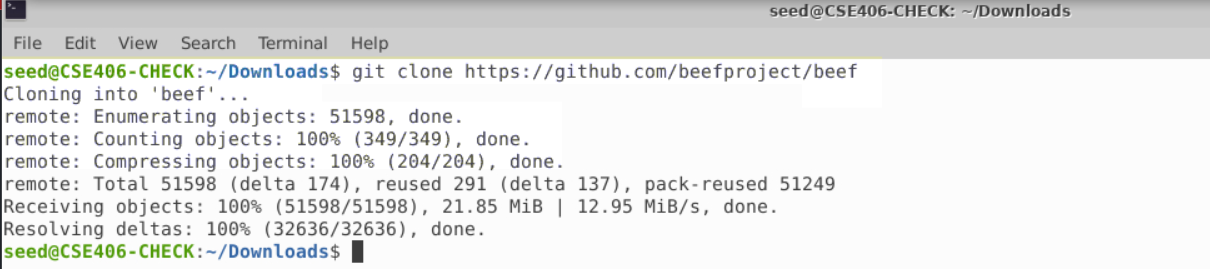
\includegraphics[width=0.80\textwidth]{Installation/install1.png}
    \caption{Cloning BeEF git repository}
    \label{fig:install1}
\end{figure}



\section{Installing BeEF}
After cloning the Git repository, navigate to the "beef" directory using the "cd beef" command, and then initiate the installation process by executing the "./install" command.


\begin{figure}[h]
    \centering
    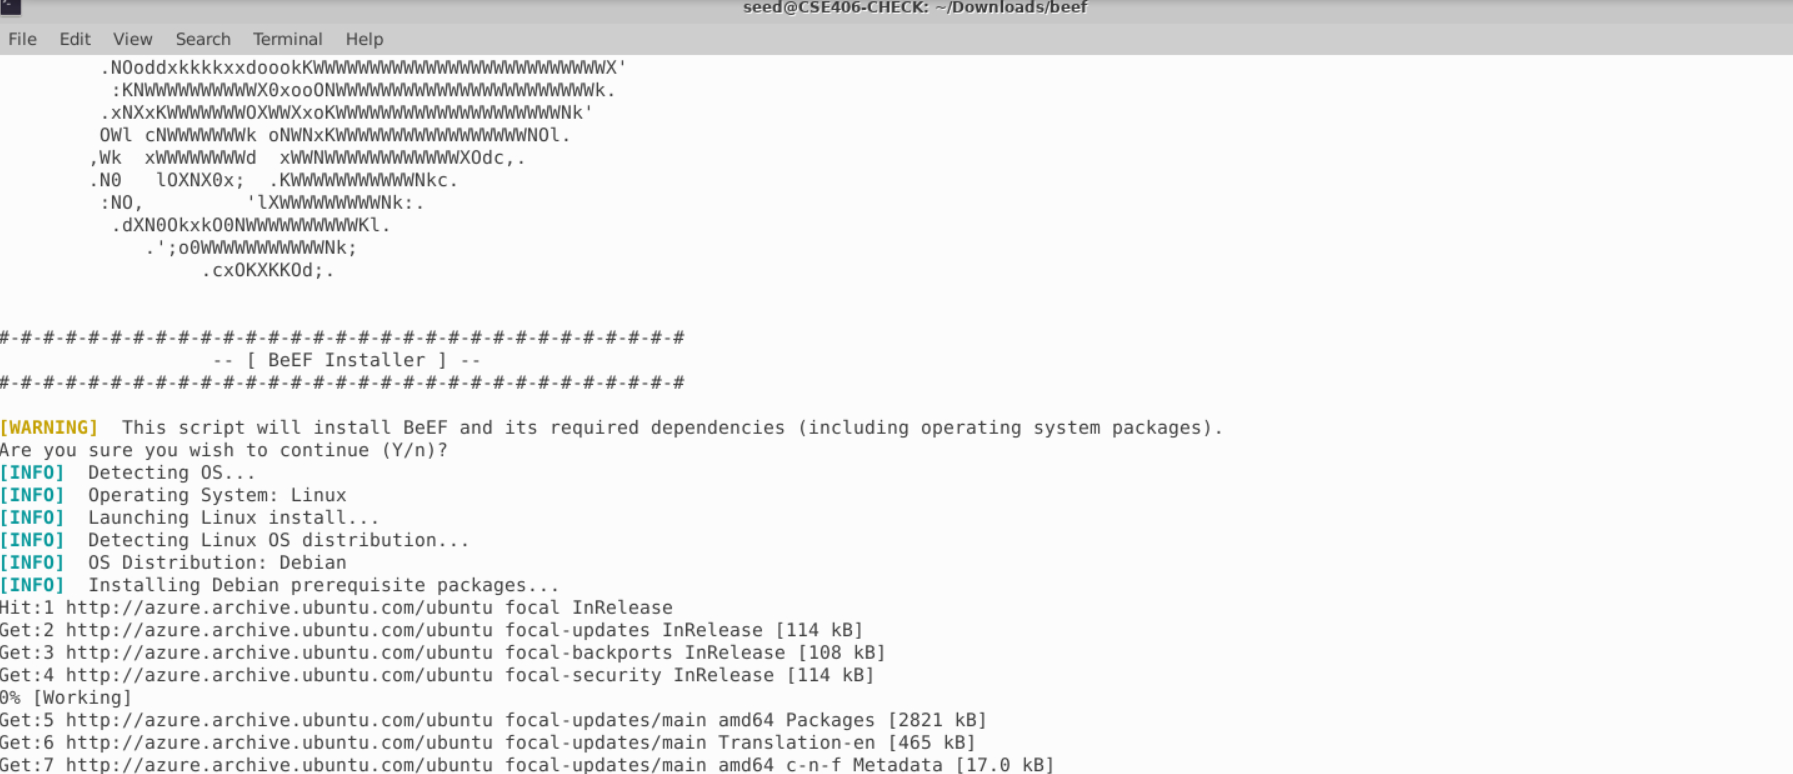
\includegraphics[width=1.0\textwidth]{Installation/install2.png}
    \caption{Installing BeEF}
    \label{fig:install2}
\end{figure}

\clearpage





\section{Configuring BeEF (credentials)}


\begin{figure}[h]
    \centering
    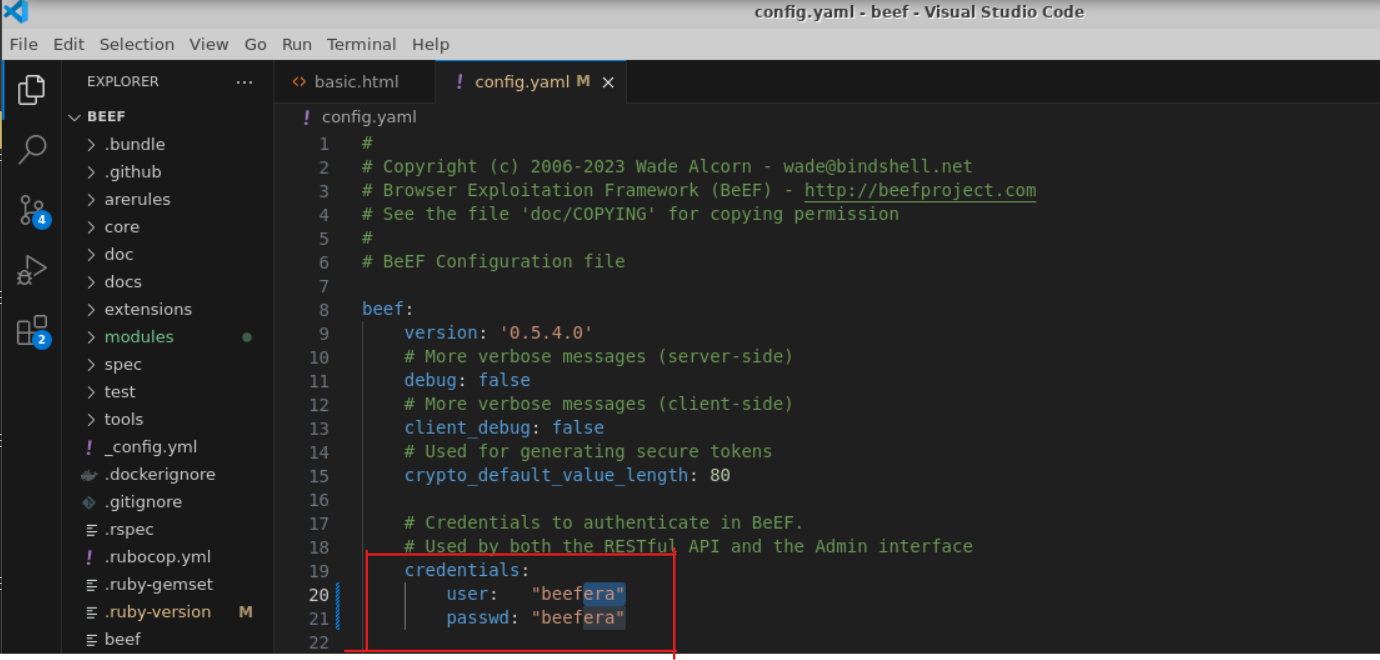
\includegraphics[width=1.0\textwidth]{Installation/install3.png}
    \caption{Configuring BeEF}
    \label{fig:}
\end{figure}

\clearpage

% \subsubsection{Sort and Filter}


\chapter{Technical design}
\begin{itemize}
    \item BeEF hook is a Javascript file, used to latch on to a target’s browser to exploit while acting as Command and control between it and the attacker.
    \item To target a web browser, first identify a webpage and then attach a BeEF hook to it
    \item Deliver javascript payload by including the javascript hook into the web page’s header.         
    \item The target browser will become hooked once they visit the site.Attacker can see all sorts of information such as plugins and extensions that the browser is using and various information about the hardware and software spaces of the target.

\end{itemize}

\section{Browser Information}
\begin{figure}[!htbp]
    \centering
    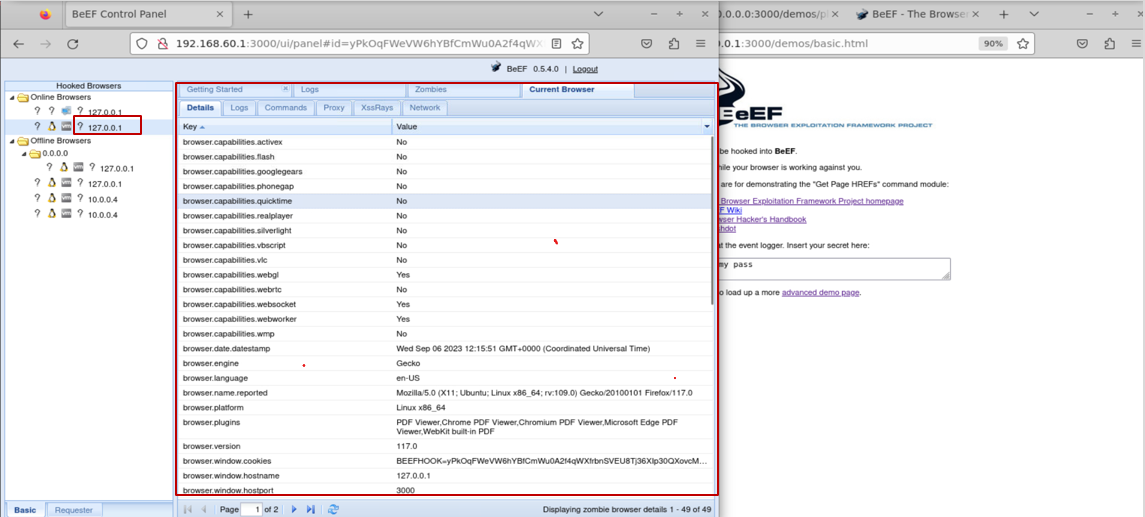
\includegraphics[width=\textwidth]{techDesign/1.png}
    \caption{Cheking Browser Information}
    \label{fig:tech1}
\end{figure}
\vfill\null

\pagebreak

\section{Logs}
It creates complete logs of mouse movements, double clicks and other actions perform by victims
\begin{figure}[!htbp]
    \centering
    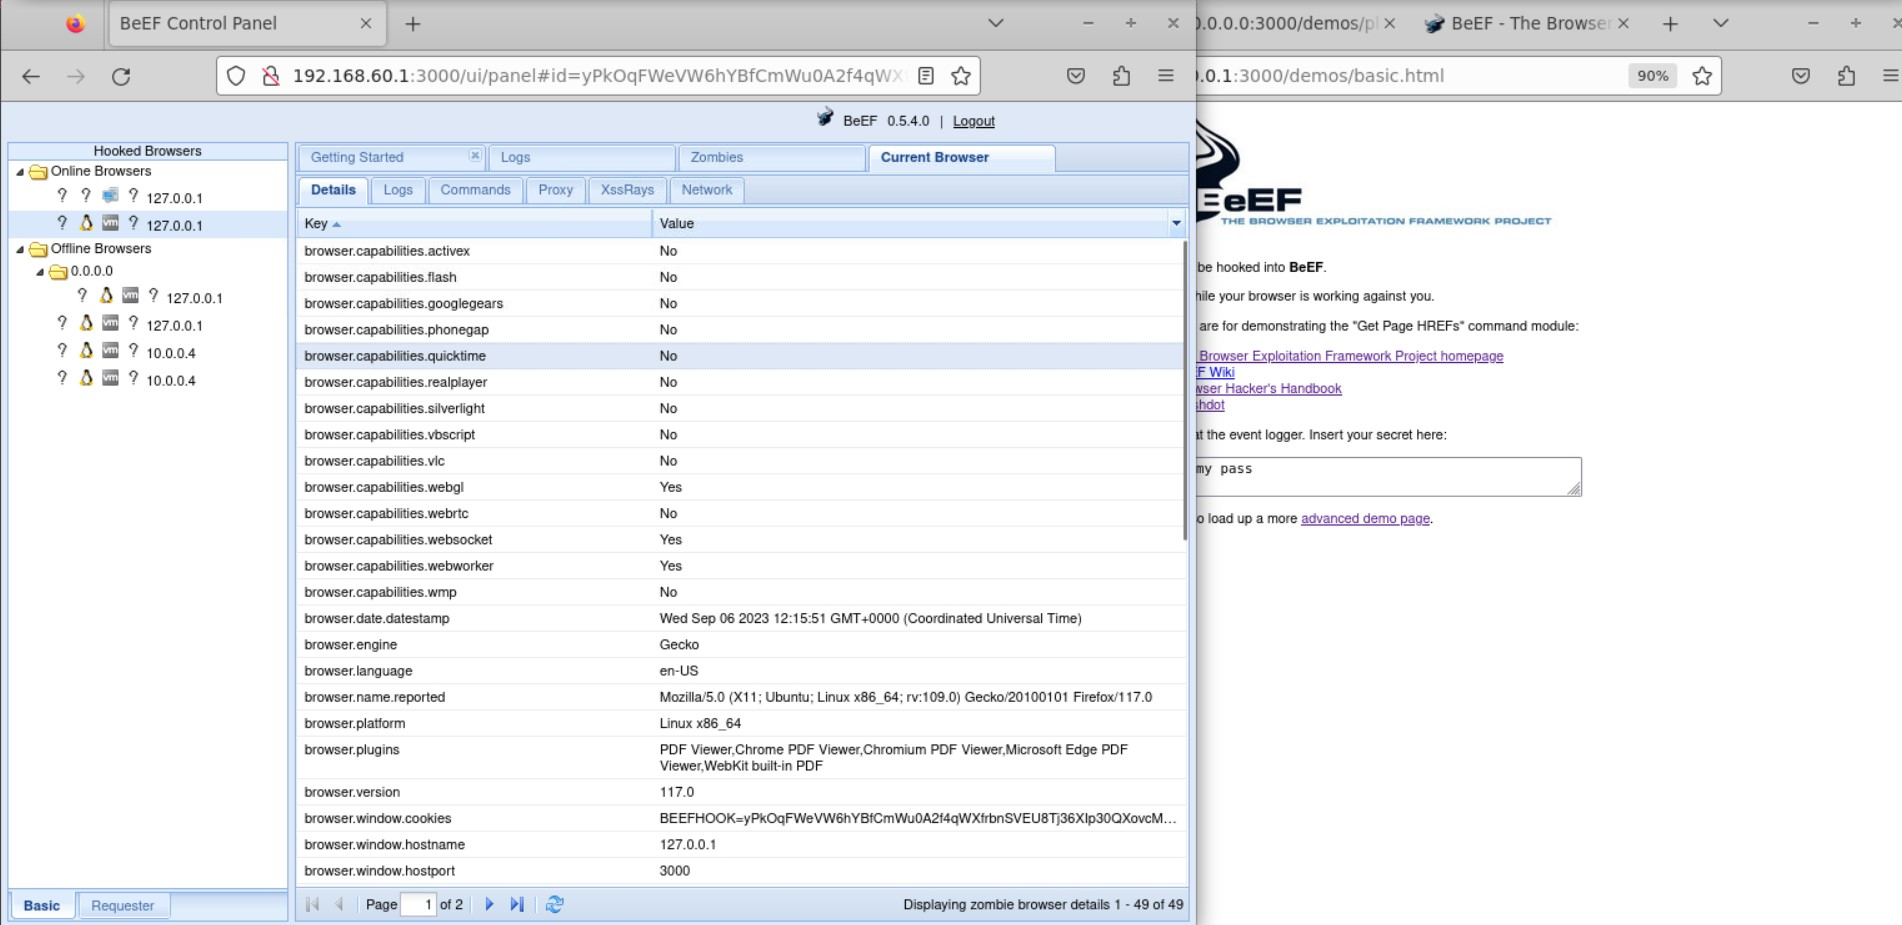
\includegraphics[width=\textwidth]{techDesign/2.png}
    \caption{Checking Log}
    \label{fig:tech2}
\end{figure}


\pagebreak


\chapter{Demonstration of some key features}

\section{Google phishing}
\subsection{Demonstration}
\begin{figure}[!htbp]
    \centering
    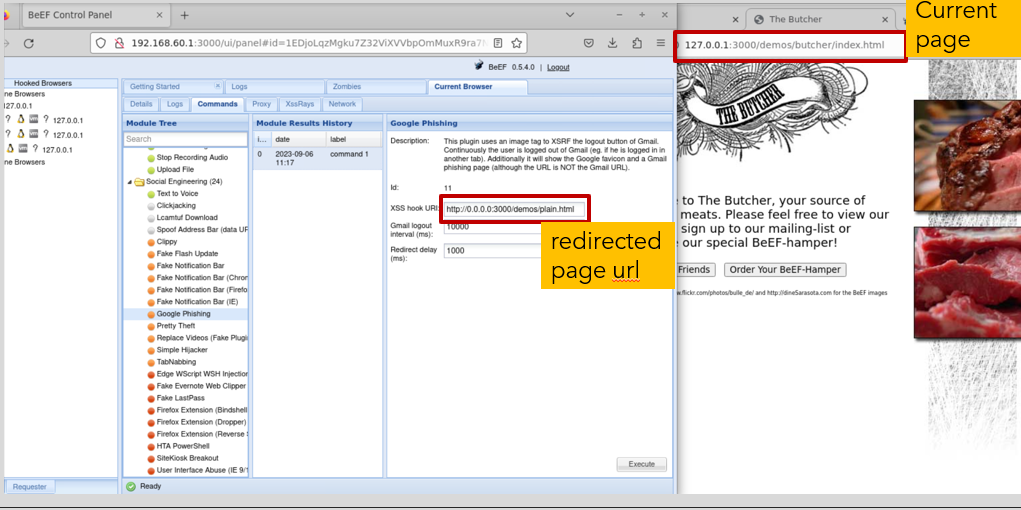
\includegraphics[width=0.8\textwidth]{google Fishing/1.png}
    \caption{Giving the hook url where the page will be redirected after  attack taking place}
    \label{fig:gp1}
\end{figure}

\begin{figure}[!htbp]
    \centering
    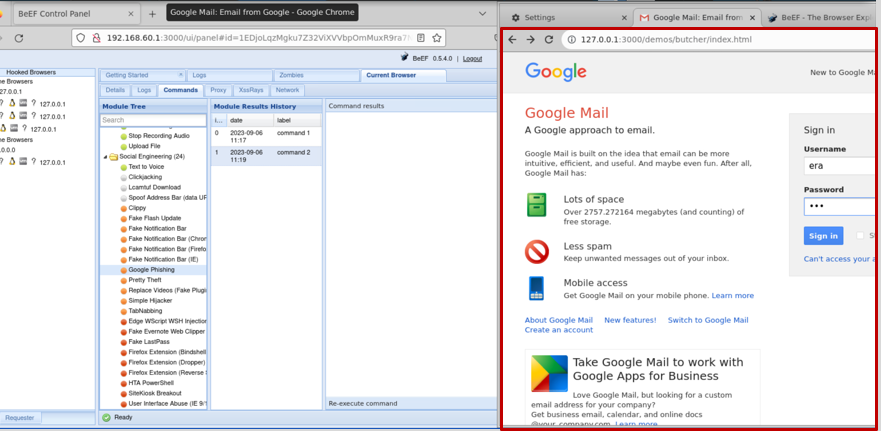
\includegraphics[width=0.8\textwidth]{google Fishing/2.png}
    \caption{Showing the fake “Sign In” page}
    \label{fig:gp2}
\end{figure}


\begin{figure}[!htbp]
    \centering
    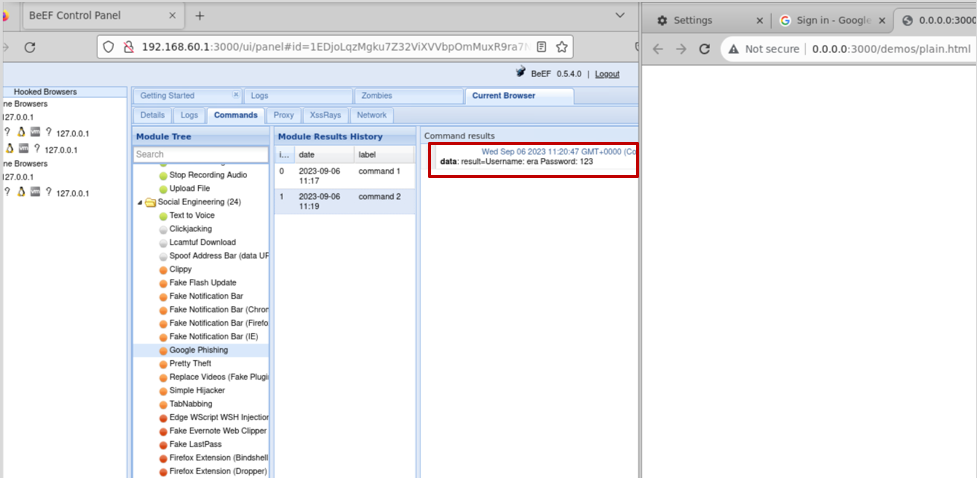
\includegraphics[width=0.8\textwidth]{google Fishing/3.png}
    \caption{Collecting user information and redirecting to another fishing url}
    \label{fig:gp3}
\end{figure}


\pagebreak

\subsection{Code}
\begin{figure}[!htbp]
    \centering
    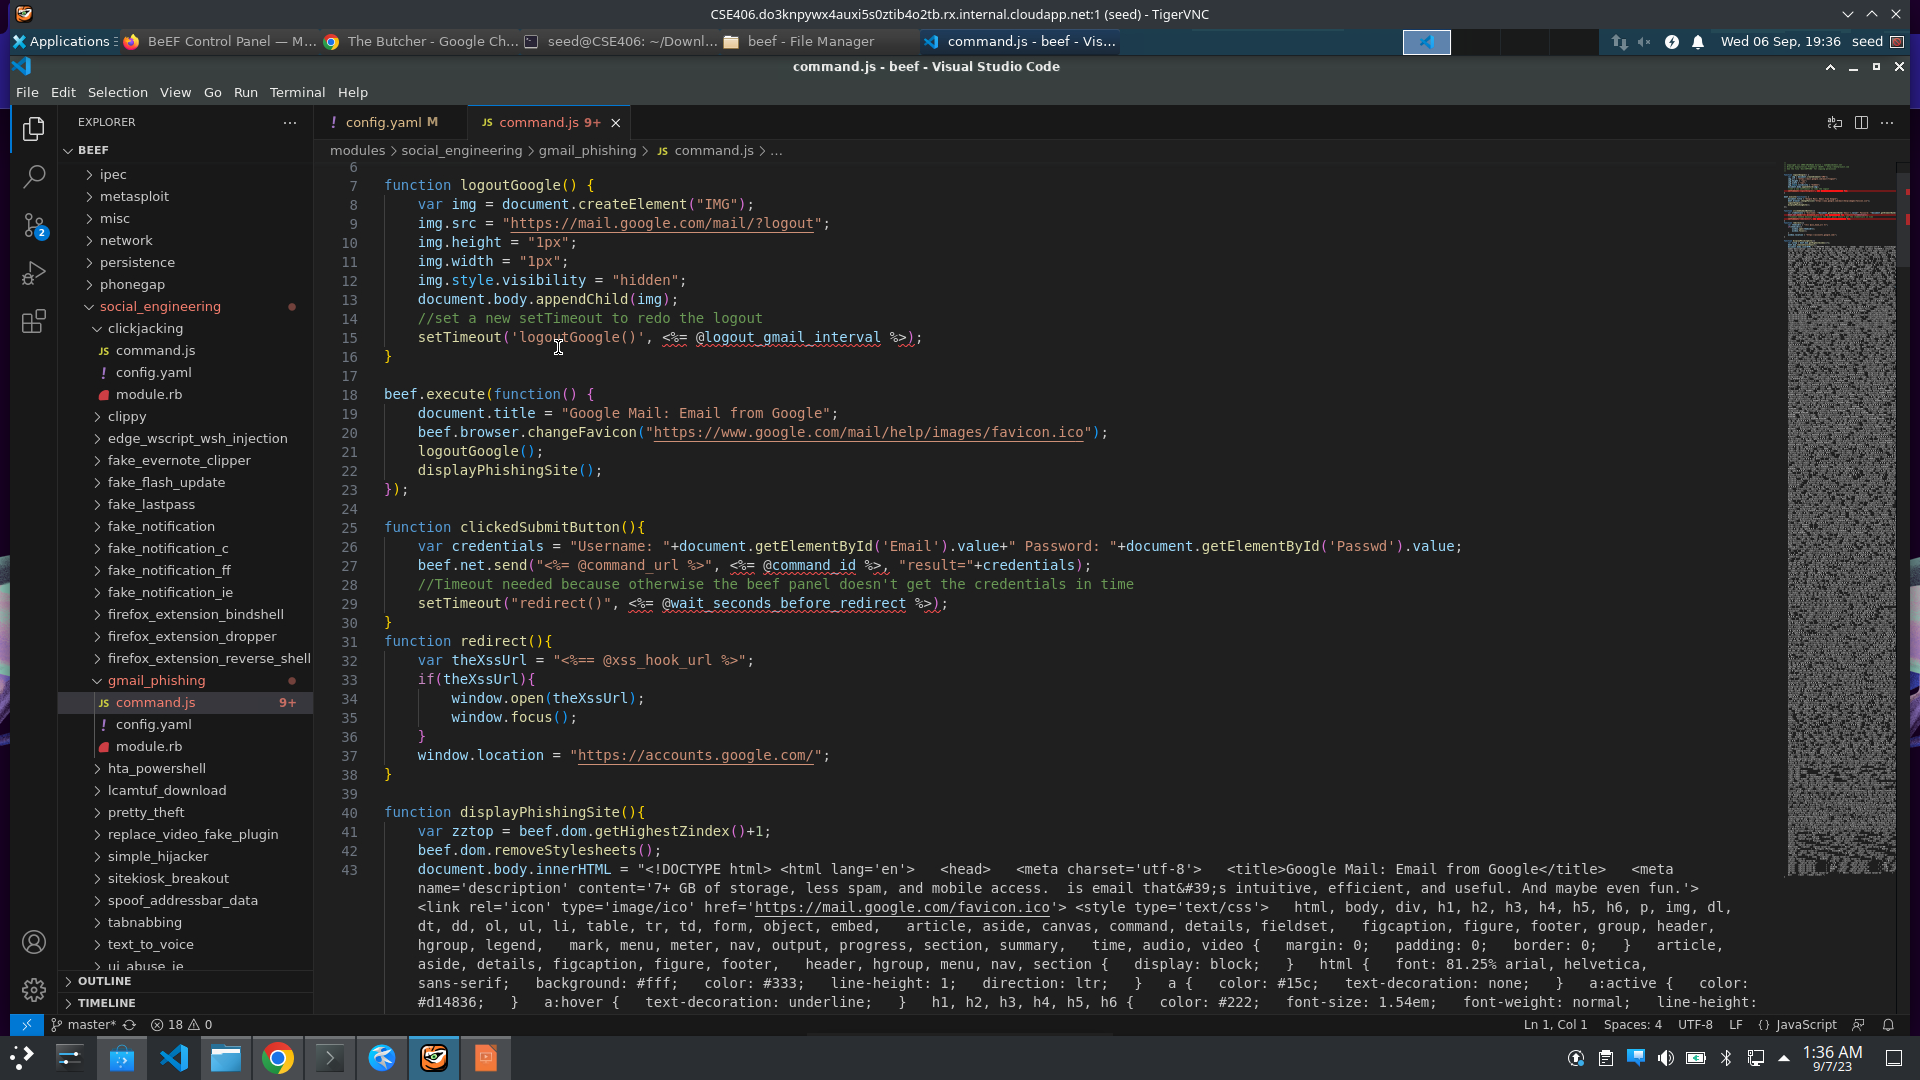
\includegraphics[width=0.8\textwidth]{google Fishing/code.png}
    \caption{Code}
    \label{fig:gp4}
\end{figure}

\pagebreak


\section{Redirect Browser}
\subsection{Demonstration}
\begin{figure}[!htbp]
    \centering
    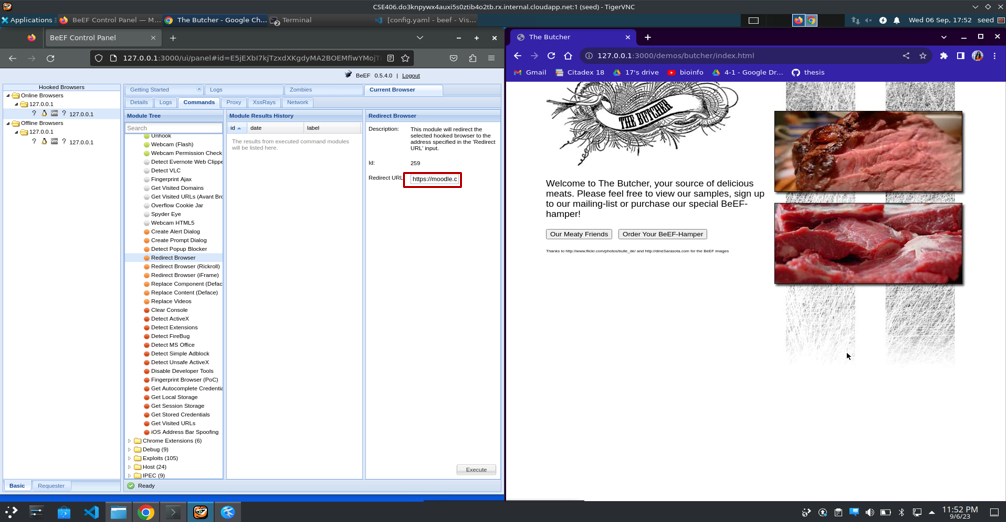
\includegraphics[width=0.8\textwidth]{Redirect Browser/1.png}
    \caption{Giving the hook url where the page will be redirected after attack taking place}
    \label{fig:rb1}
\end{figure}

\begin{figure}[!htbp]
    \centering
    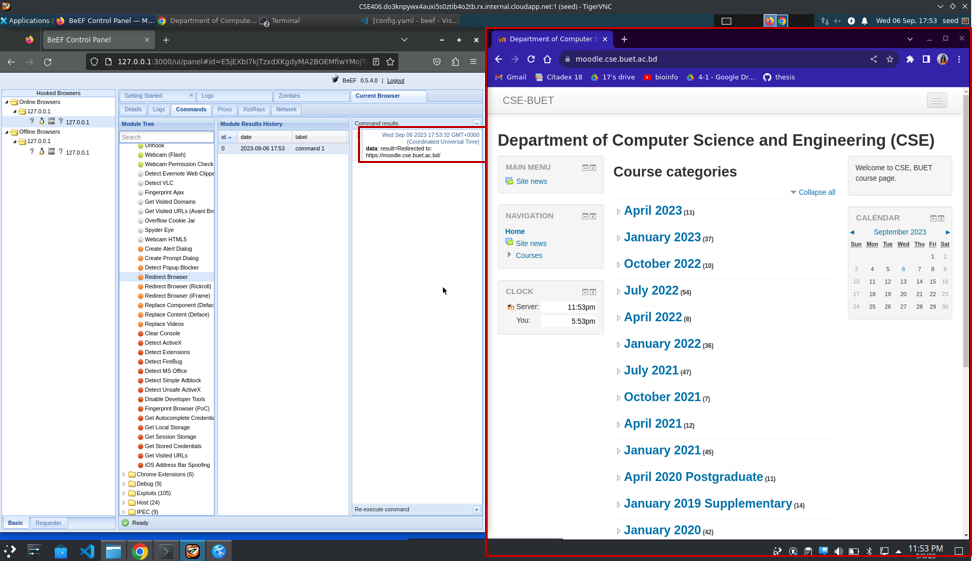
\includegraphics[width=0.8\textwidth]{Redirect Browser/2.png}
    \caption{Redirecting to the phishing site}
    \label{fig:rb2}
\end{figure}

\pagebreak

\subsection{Code}
\begin{figure}[!htbp]
    \centering
    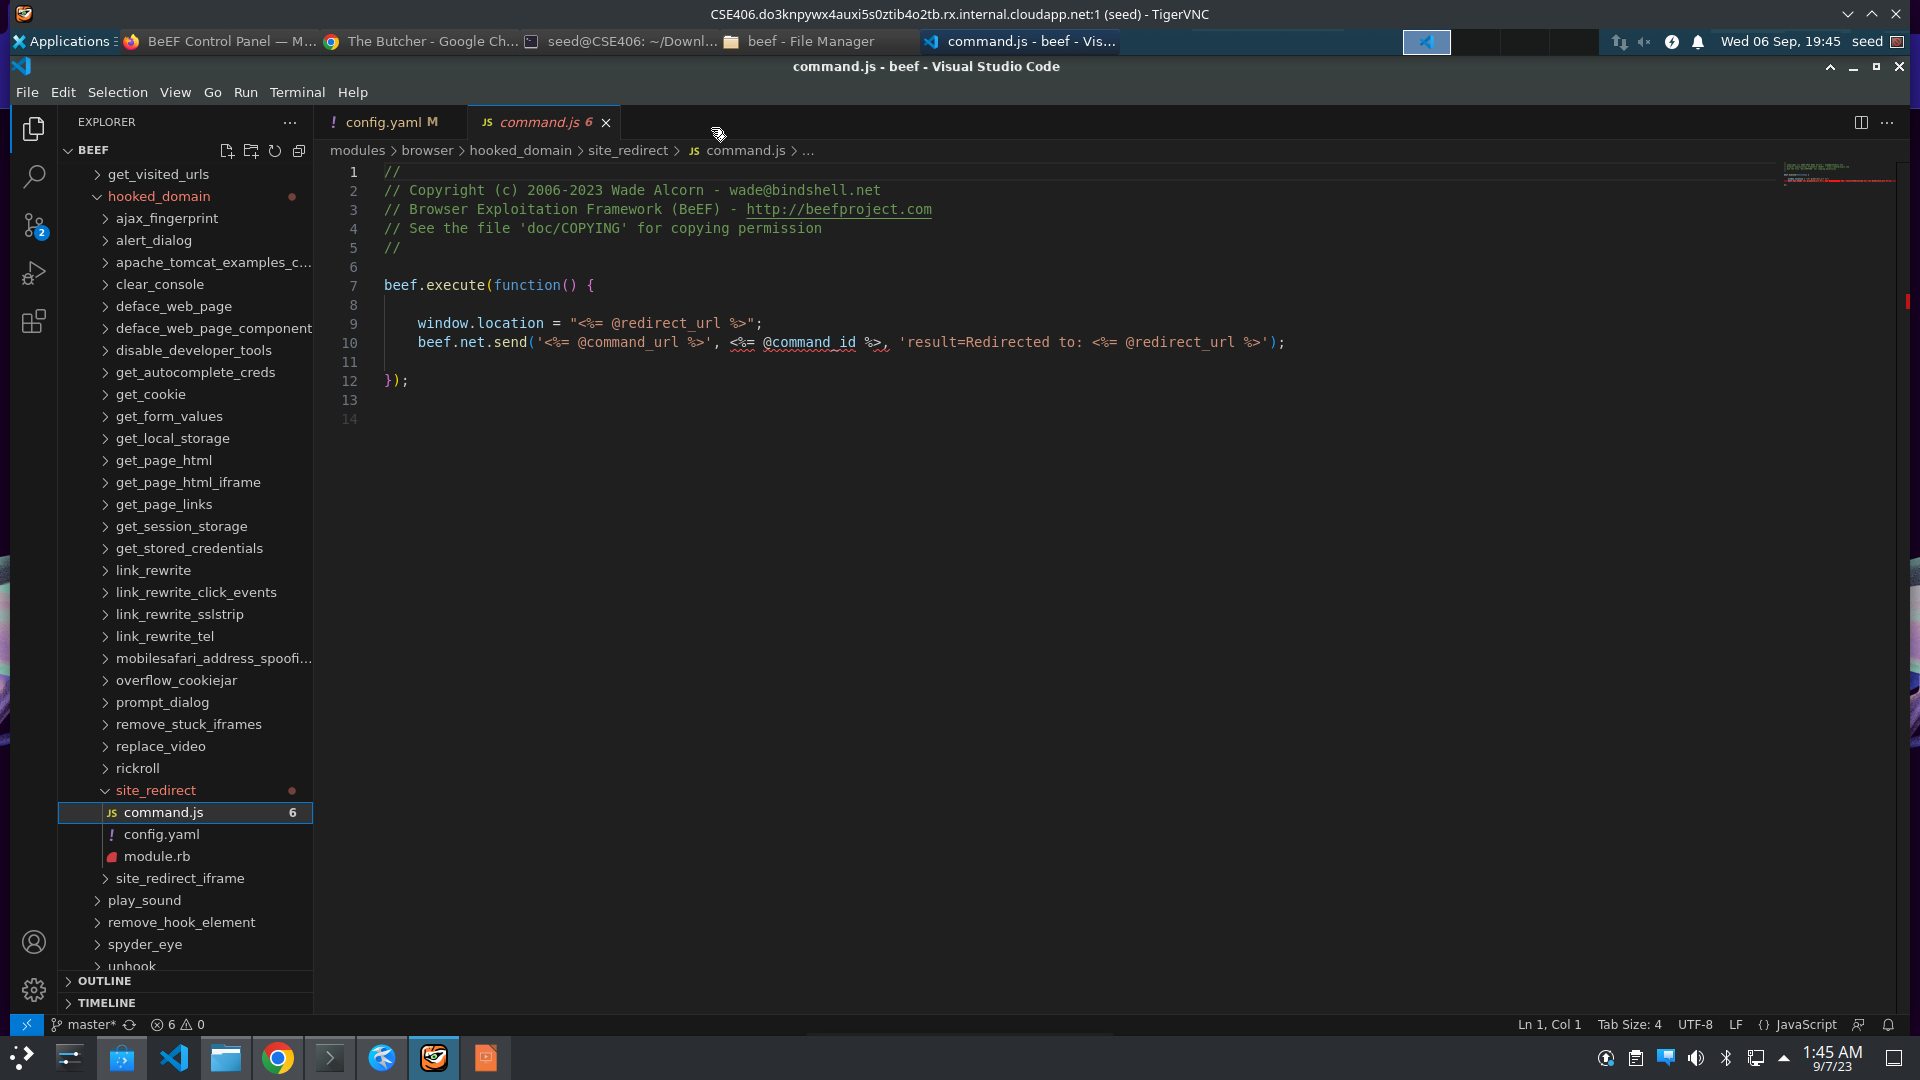
\includegraphics[width=0.8\textwidth]{Redirect Browser/code.png}
    \caption{Code}
    \label{fig:rb3}
\end{figure}

\pagebreak

\section{Redirect Browser(Rickroll)}
\subsection{Demonstration}
\begin{figure}[!htbp]
    \centering
    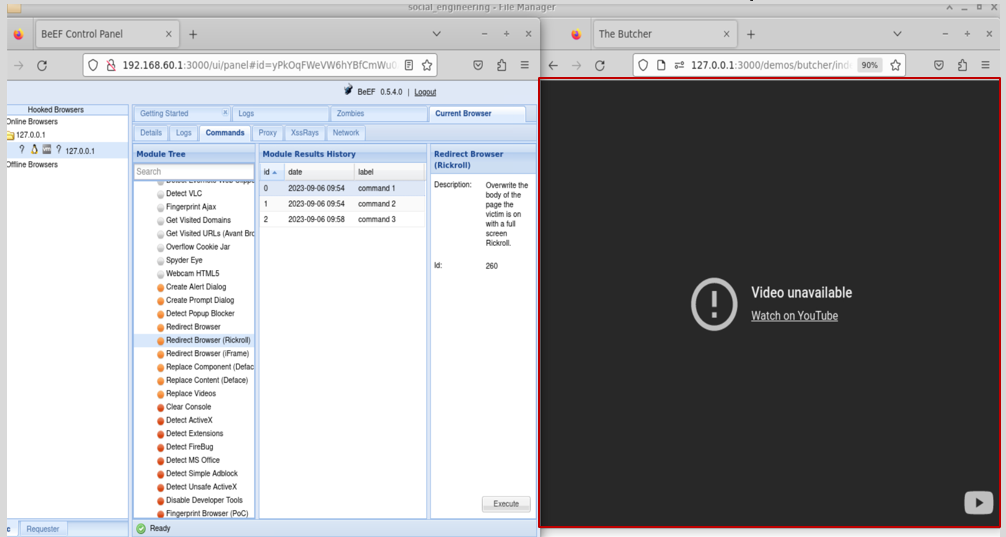
\includegraphics[width=0.8\textwidth]{Redirect Browser(Rickroll)/1.png}
    \caption{Overwriting the body of the page with a full screen rickroll}
    \label{fig:rr1}
\end{figure}

\begin{figure}[!htbp]
    \centering
    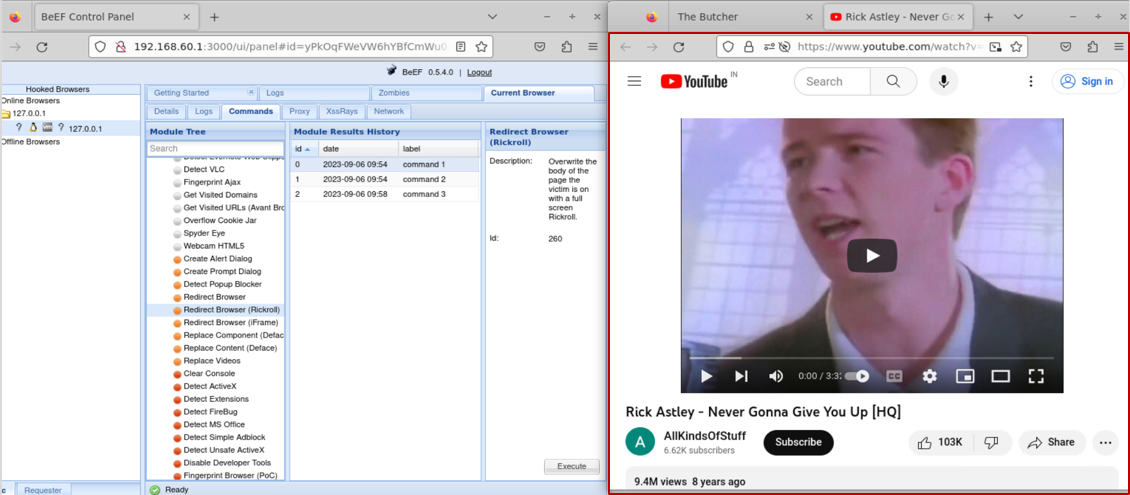
\includegraphics[width=0.8\textwidth]{Redirect Browser(Rickroll)/2.png}
    \caption{Redirecting to video}
    \label{fig:rr2}
\end{figure}

\pagebreak

\subsection{Code}
\begin{figure}[!htbp]
    \centering
    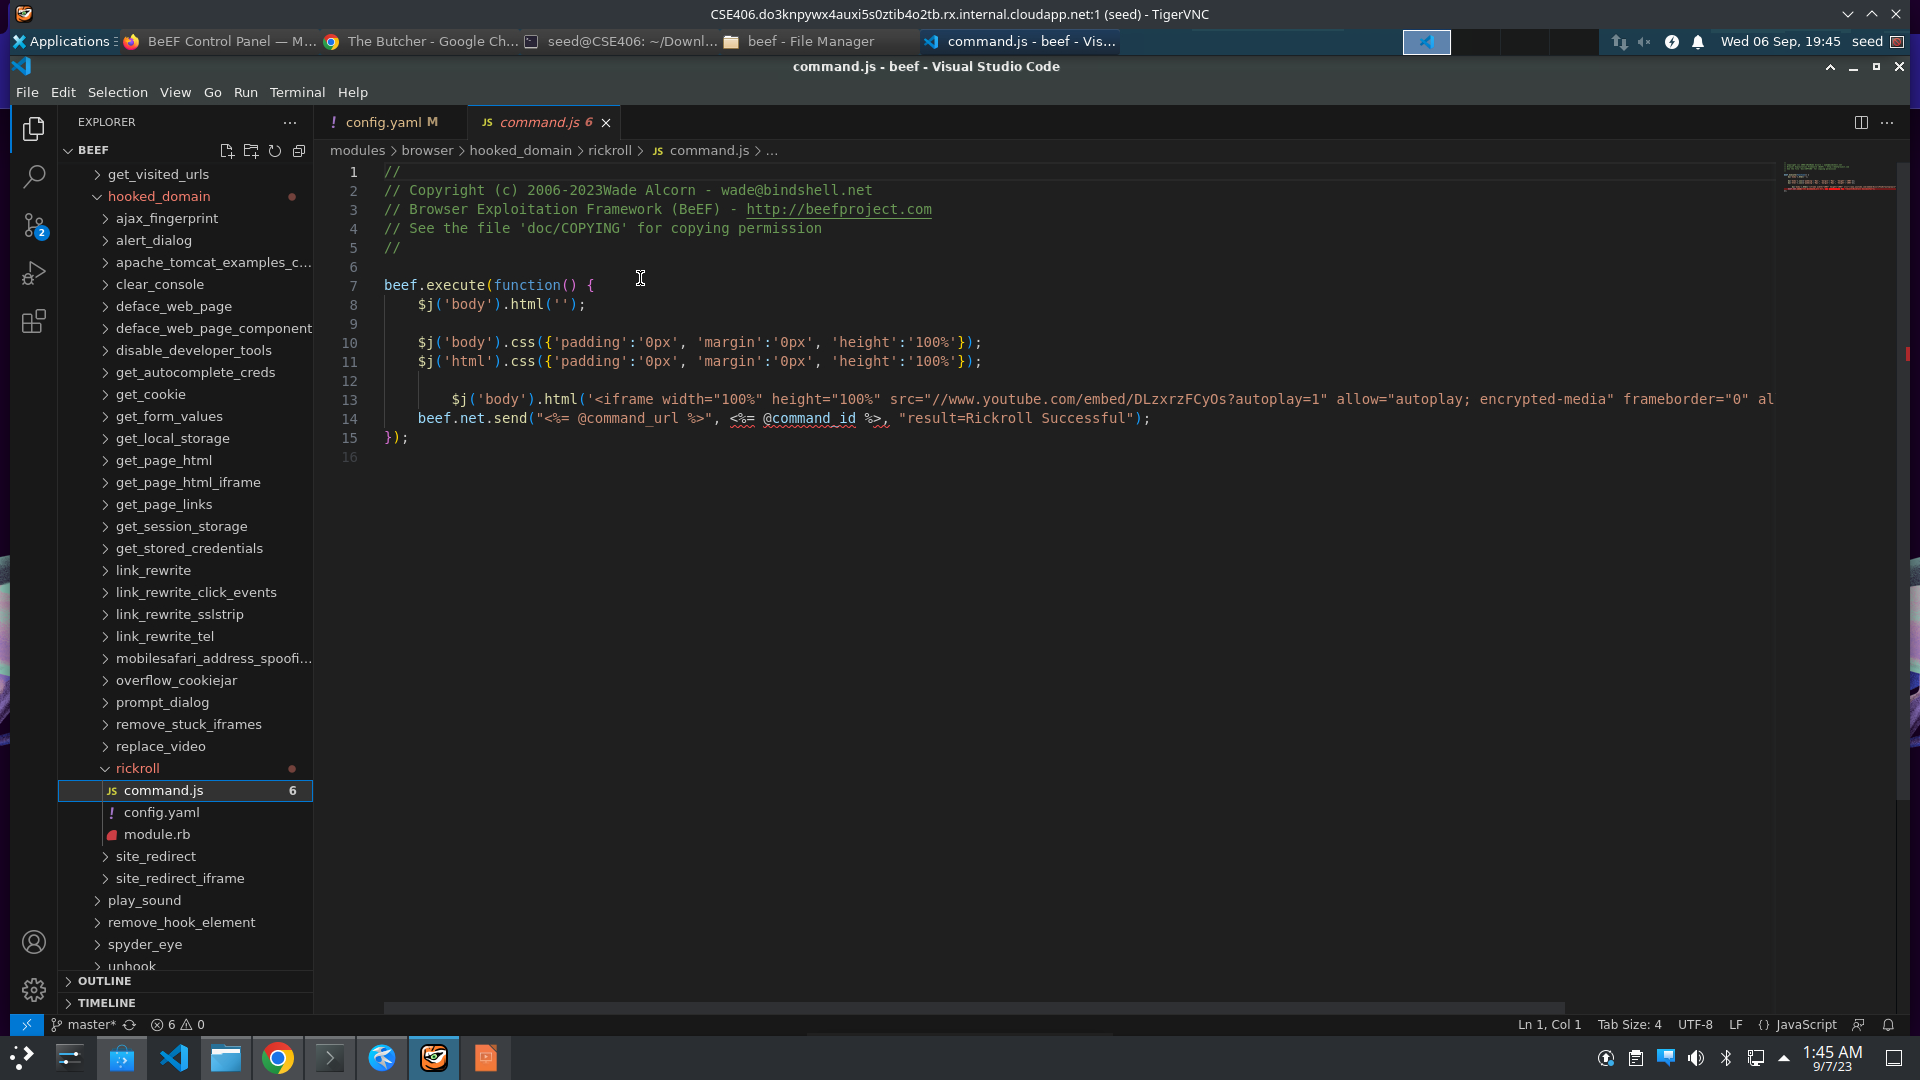
\includegraphics[width=0.8\textwidth]{Redirect Browser(Rickroll)/code.png}
    \caption{Code}
    \label{fig:rr3}
\end{figure}

\pagebreak

\section{Alert Dialog}
\subsection{Demonstration}

\begin{figure}[!htbp]
    \centering
    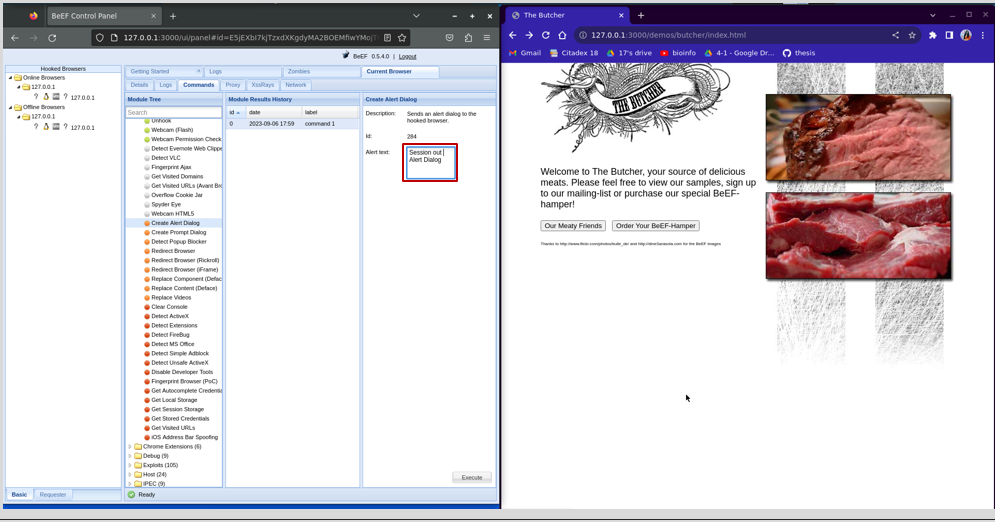
\includegraphics[width=0.8\textwidth]{Alert Dialog/1.png}
    \caption{fake alert message to user}
    \label{fig:ad1}
\end{figure}

\begin{figure}[!htbp]
    \centering
    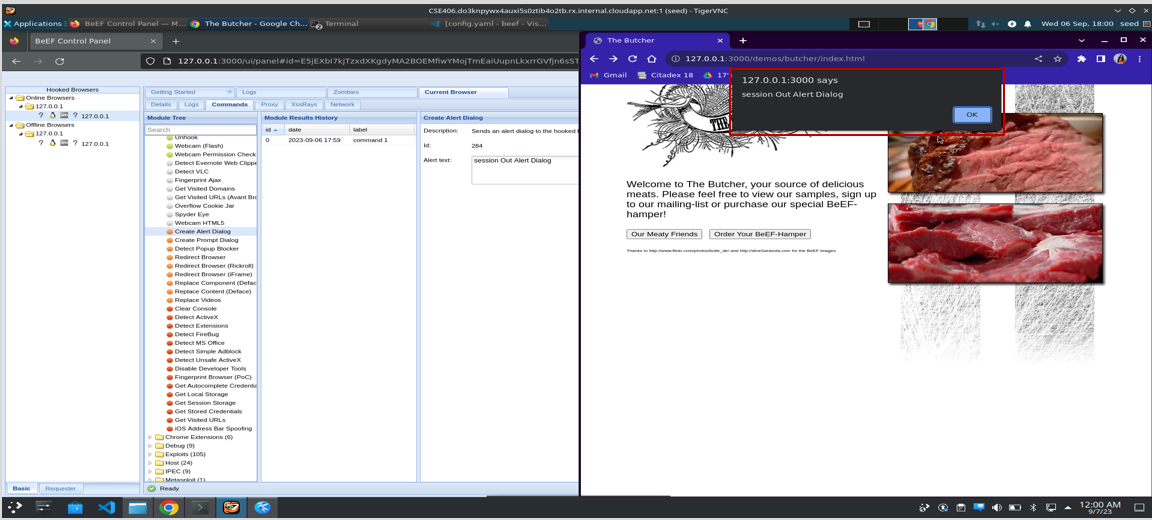
\includegraphics[width=0.8\textwidth]{Alert Dialog/2.png}
    \caption{fake message sent}
    \label{fig:ad2}
\end{figure}

\pagebreak

\subsection{Code}
\begin{figure}[!htbp]
    \centering
    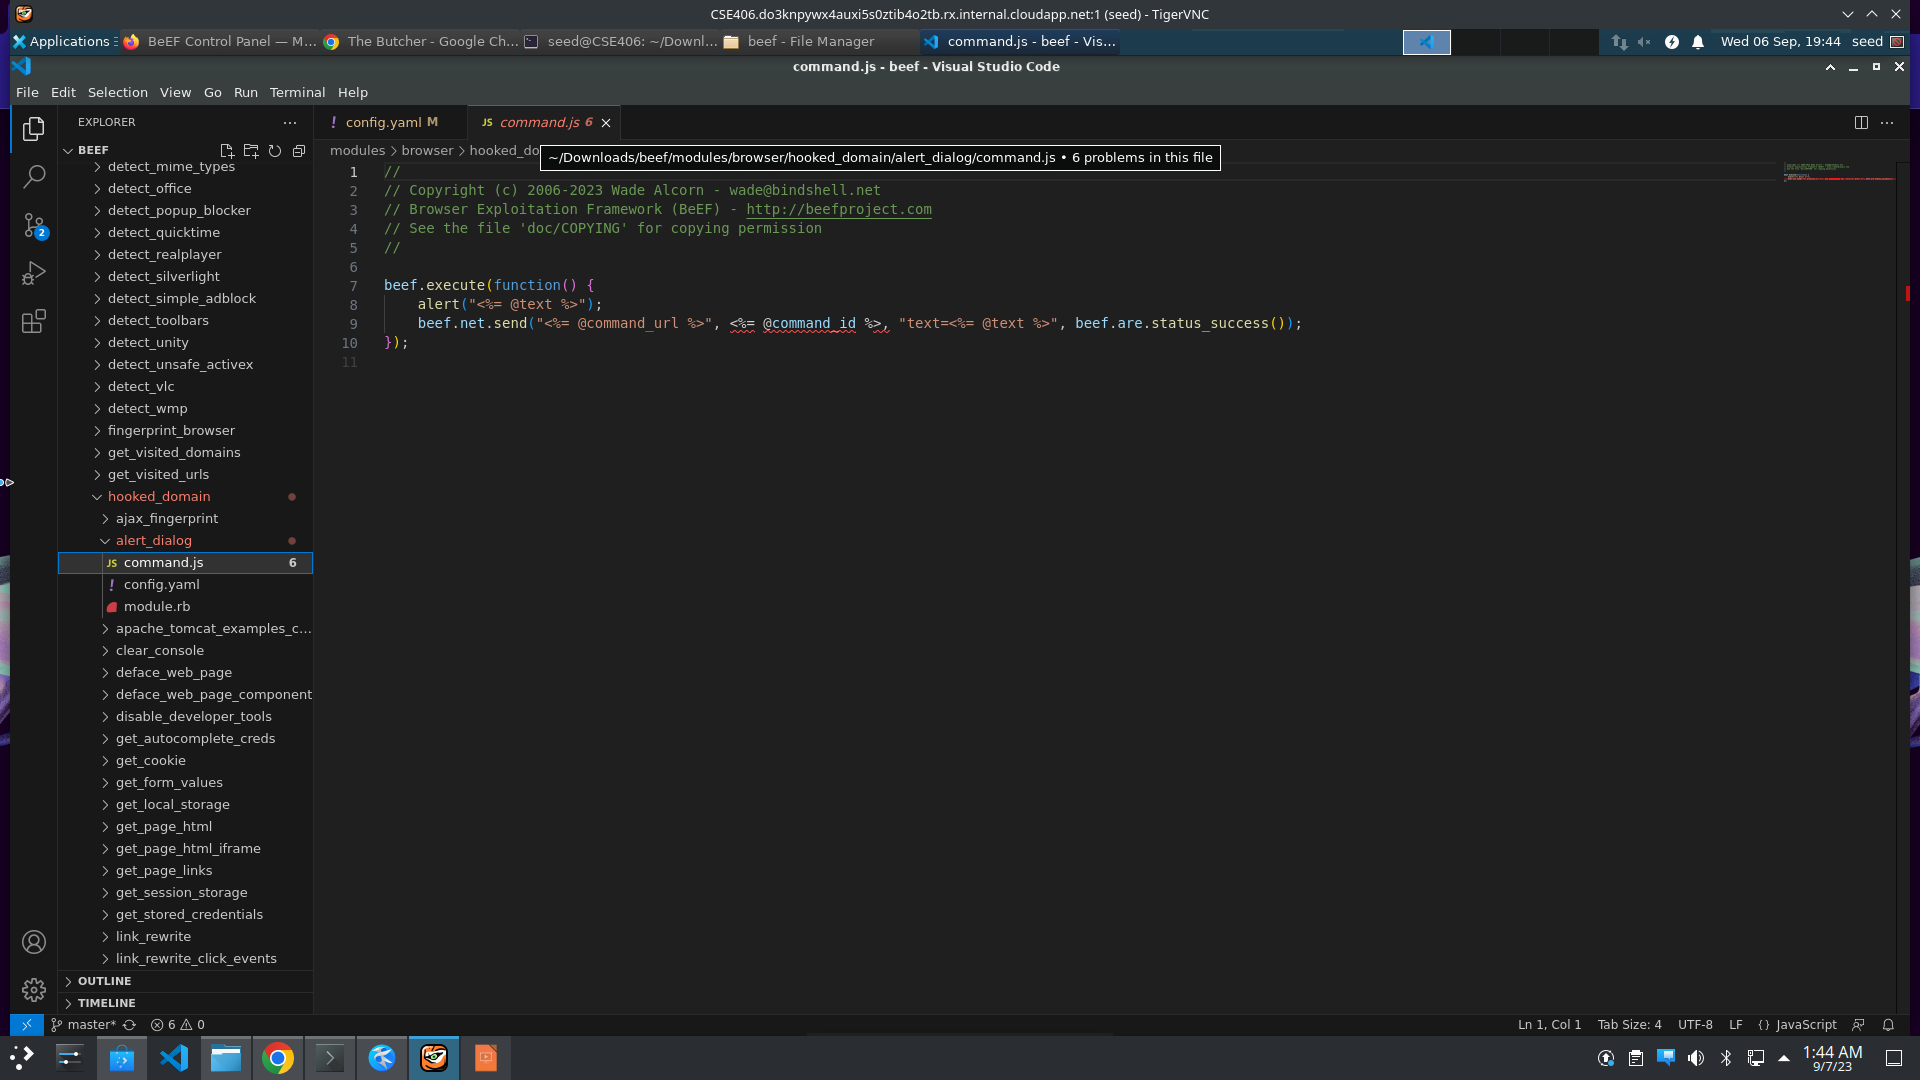
\includegraphics[width=0.8\textwidth]{Alert Dialog/code.png}
    \caption{Code}
    \label{fig:ad3}
\end{figure}

\pagebreak


\section{Get Cookie}
\subsection{Demonstration}

\begin{figure}[!htbp]
    \centering
    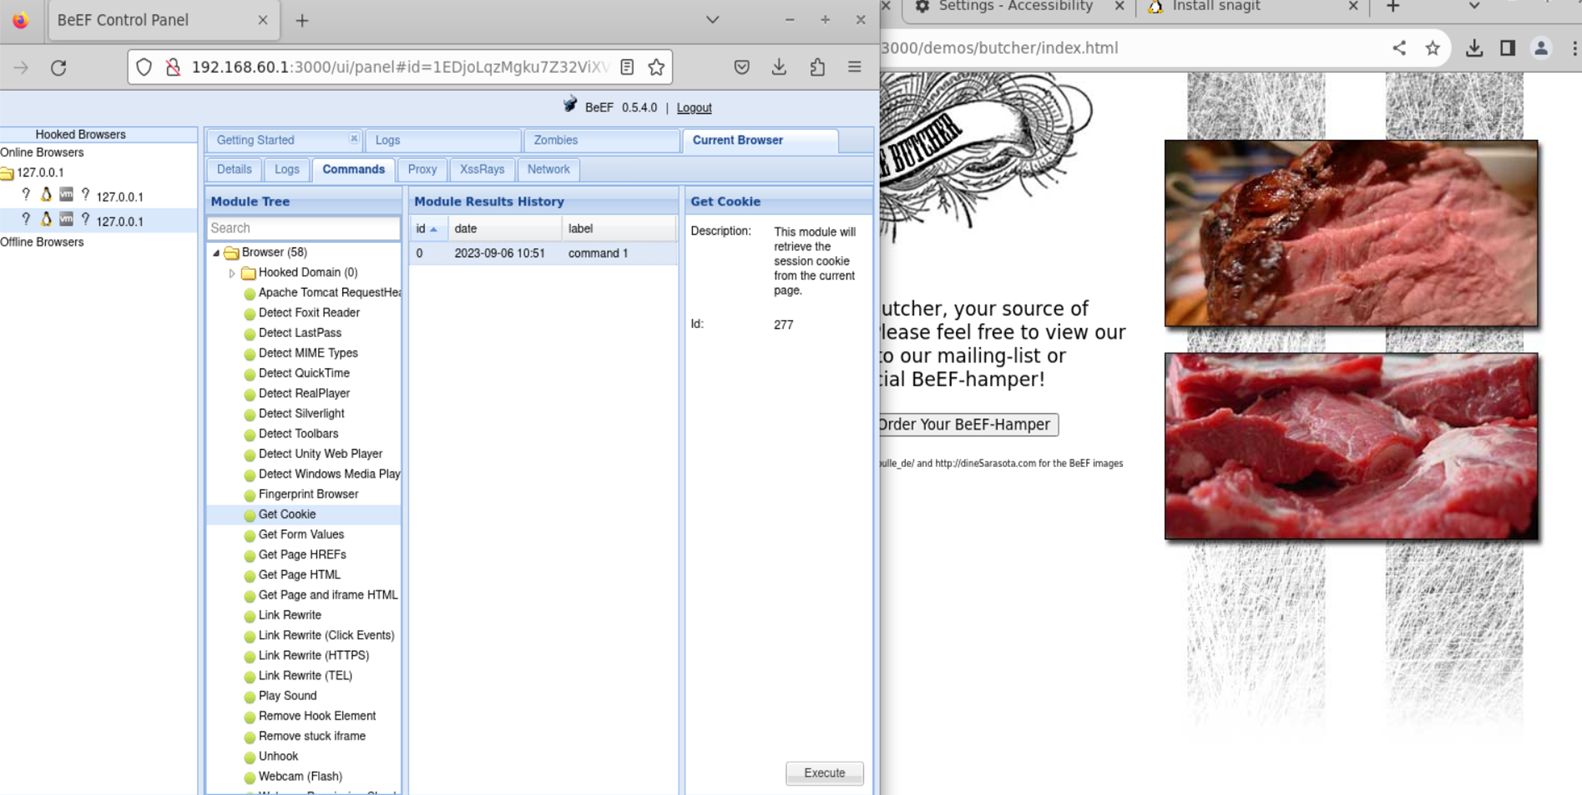
\includegraphics[width=0.8\textwidth]{Get Cookie/1.png}
    \caption{Retrieving current session cookies}
    \label{fig:gc1}
\end{figure}

\begin{figure}[!htbp]
    \centering
    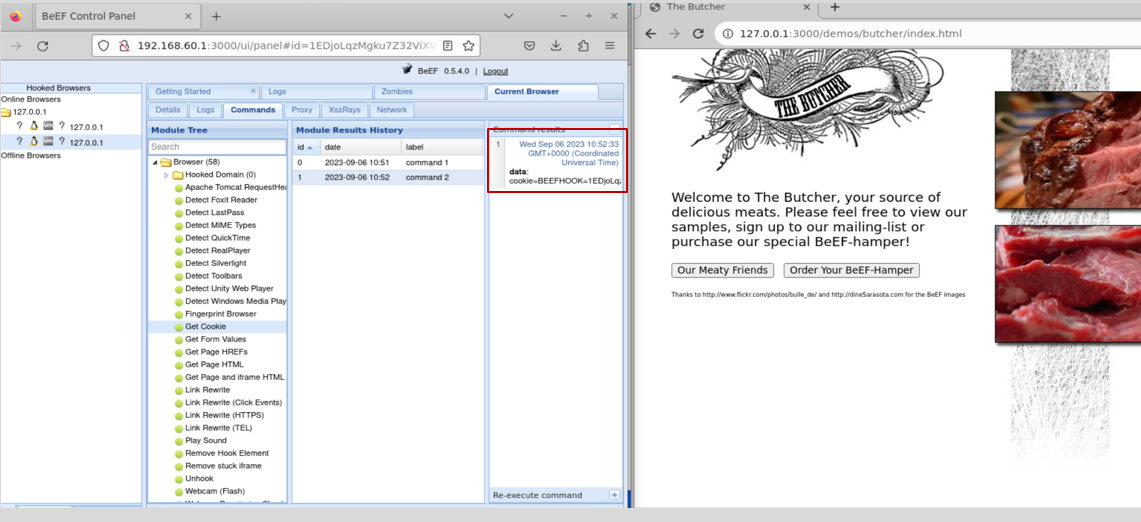
\includegraphics[width=0.8\textwidth]{Get Cookie/2.png}
    \caption{Getting session cookies}
    \label{fig:gc2}
\end{figure}

\pagebreak

\subsection{Code}
\begin{figure}[!htbp]
    \centering
    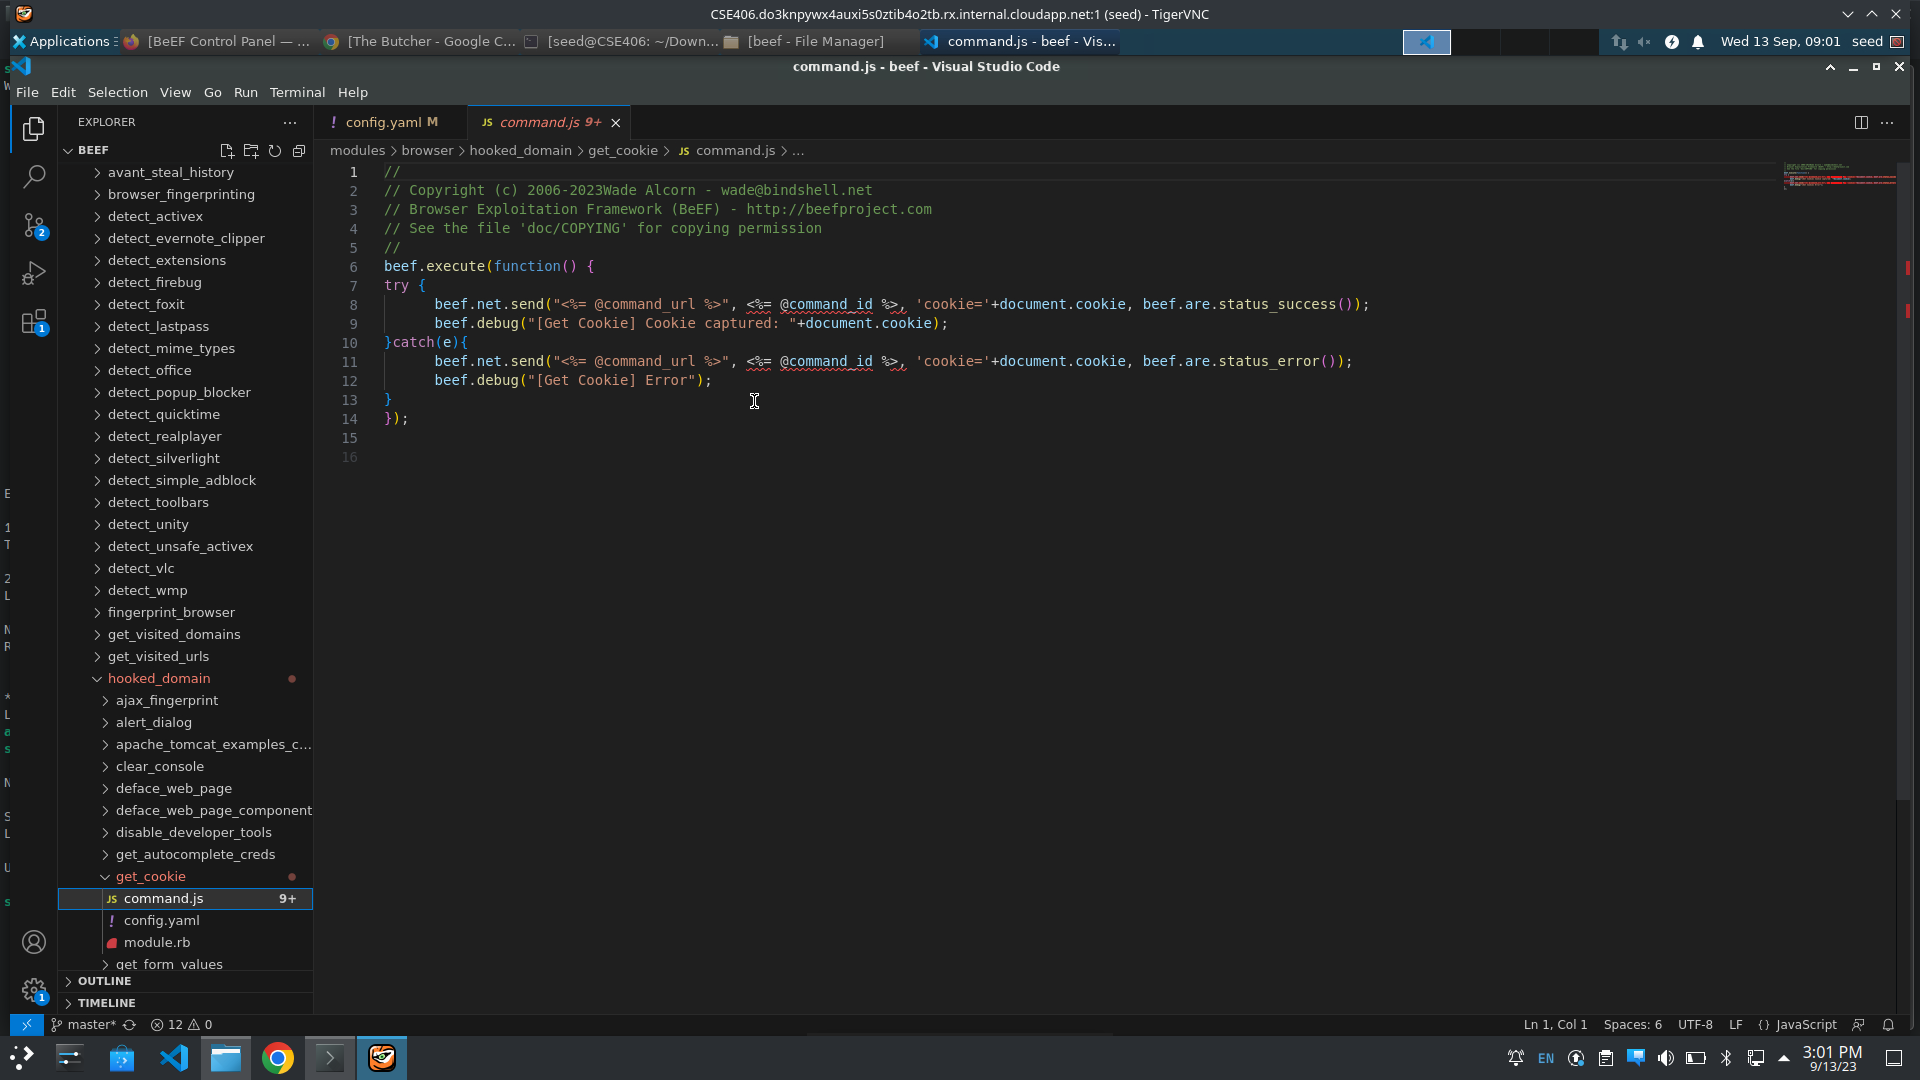
\includegraphics[width=0.8\textwidth]{Get Cookie/code.png}
    \caption{Code}
    \label{fig:gc3}
\end{figure}

\pagebreak


\section{TabNabbing}
\subsection{Demonstration}

\begin{figure}[!htbp]
    \centering
    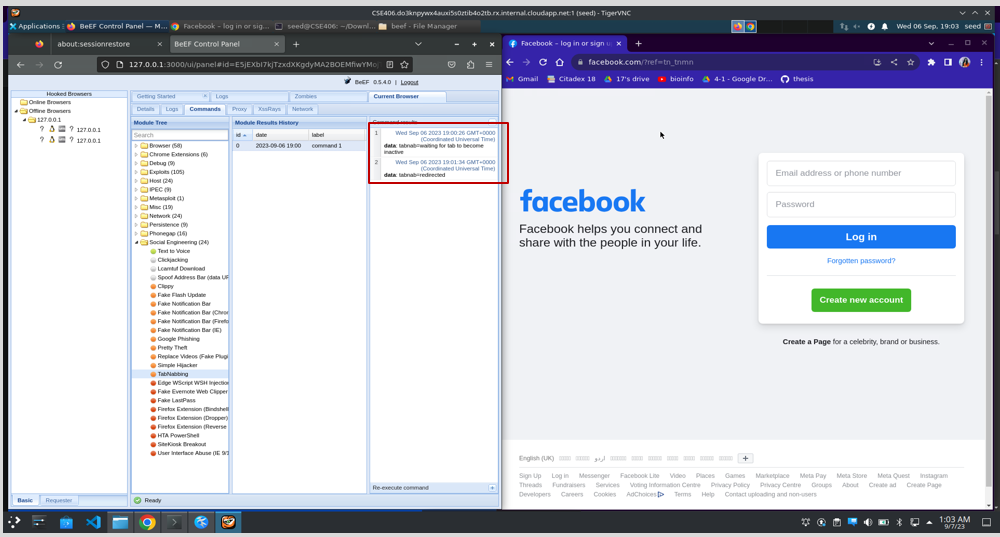
\includegraphics[width=0.8\textwidth]{TabNabbing/1.png}
    \caption{Redirects to the specified URL after the tab has been inactive for a specified amount of time}
    \label{fig:tn1}
\end{figure}

\subsection{Code}
\begin{figure}[!htbp]
    \centering
    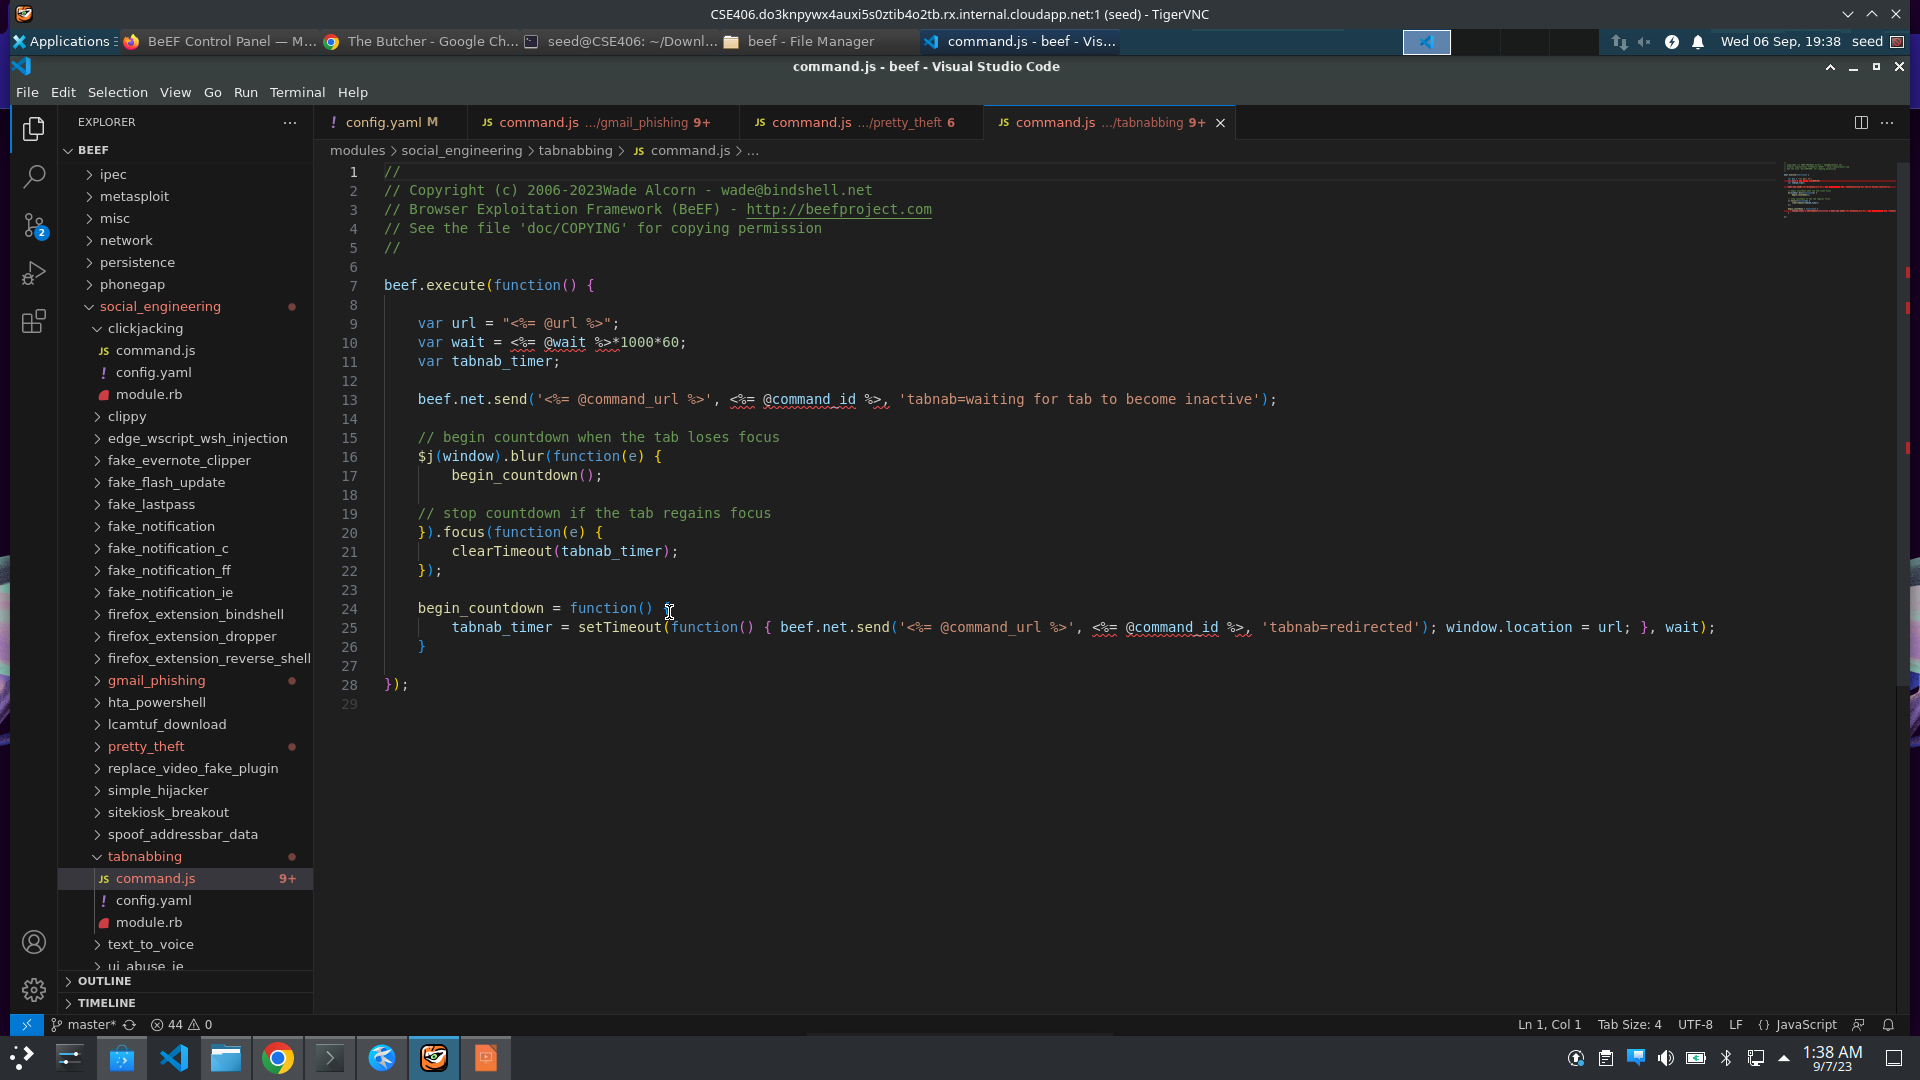
\includegraphics[width=0.8\textwidth]{TabNabbing/code.png}
    \caption{Code}
    \label{fig:tn2}
\end{figure}

\pagebreak

\section{Fake Notification}
\subsection{Demonstration}

\begin{figure}[!htbp]
    \centering
    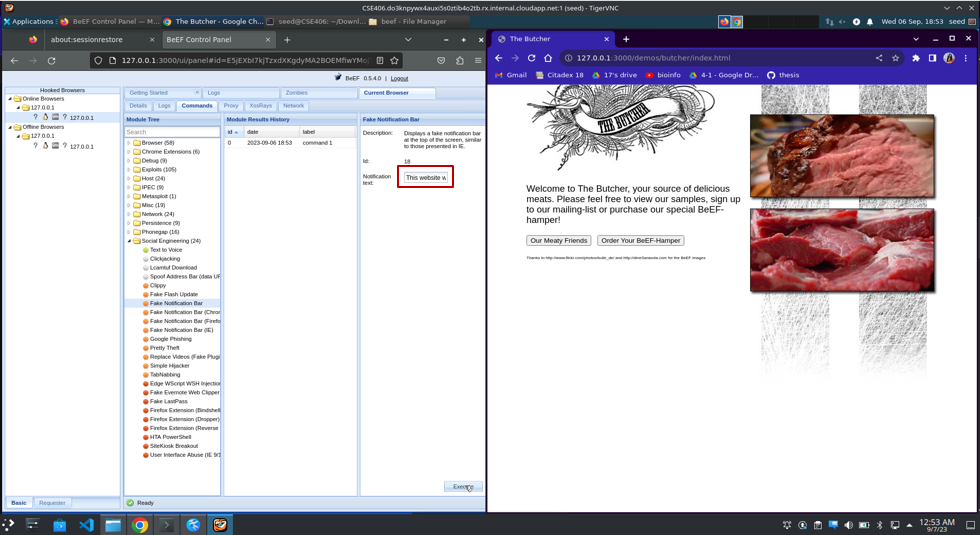
\includegraphics[width=0.8\textwidth]{Fake Notification Bar/1.png}
    \caption{Displays fake notification bar at the top of screen}
    \label{fig:fn1}
\end{figure}

\begin{figure}[!htbp]
    \centering
    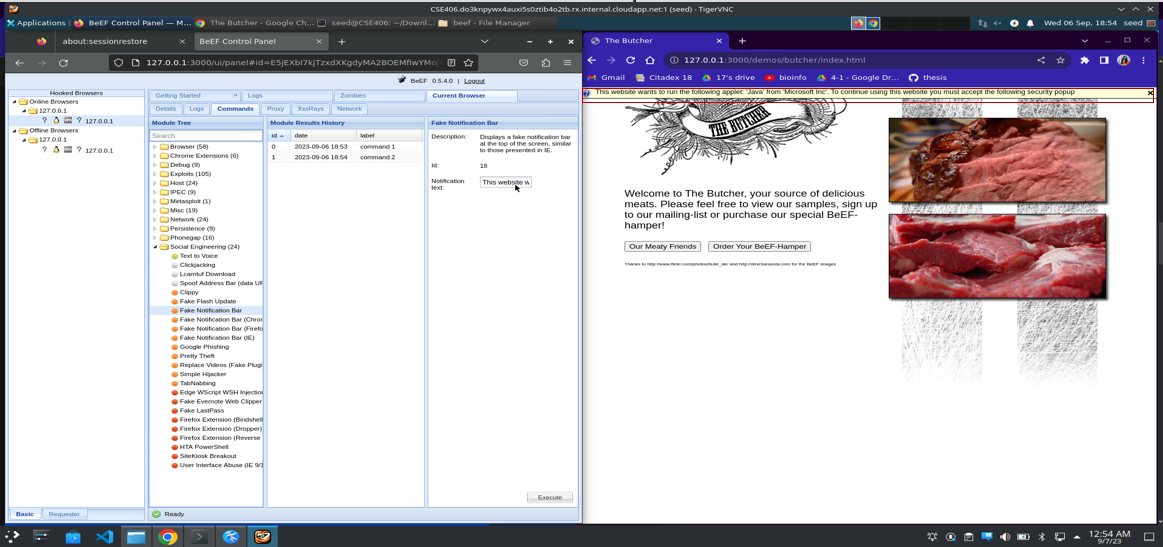
\includegraphics[width=0.8\textwidth]{Fake Notification Bar/2.png}
    \caption{Notification sent}
    \label{fig:fn2}
\end{figure}

\pagebreak

\subsection{Code}
\begin{figure}[!htbp]
    \centering
    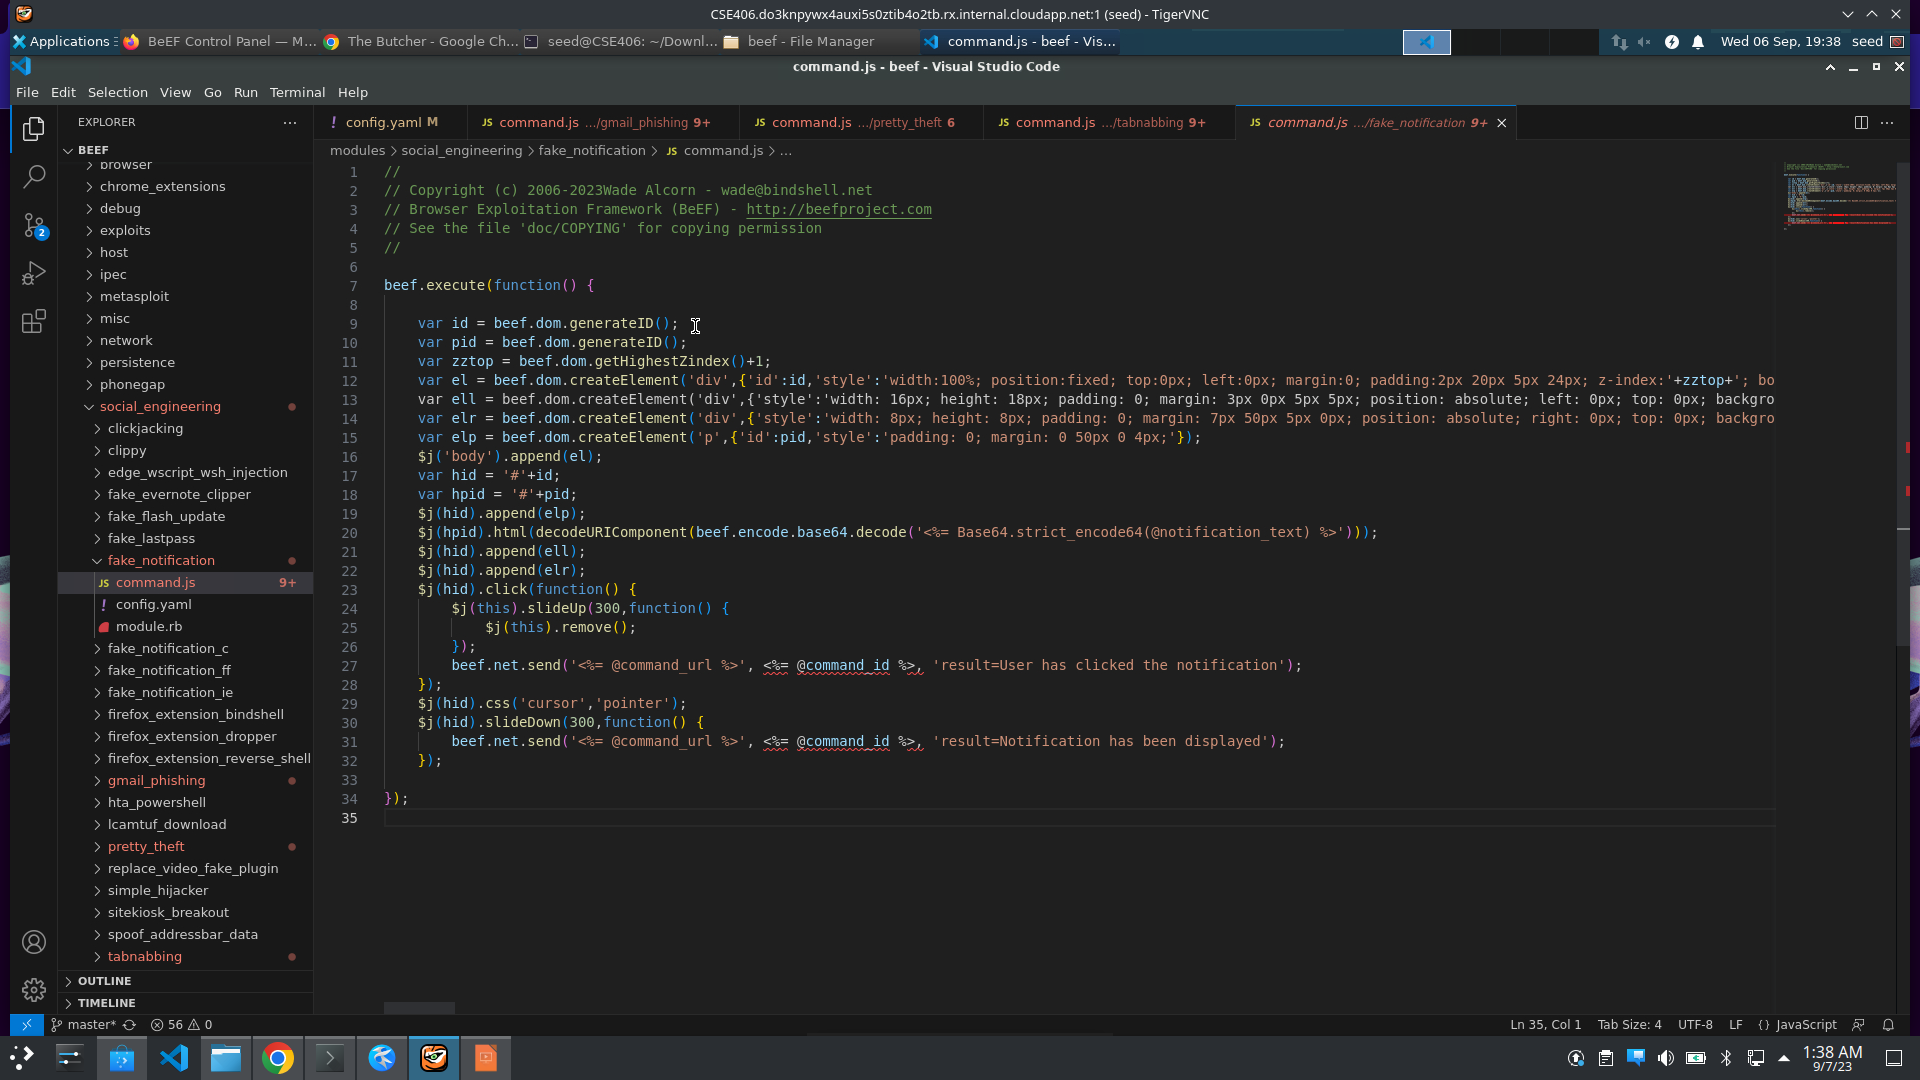
\includegraphics[width=0.8\textwidth]{Fake Notification Bar/code.png}
    \caption{Code}
    \label{fig:fn3}
\end{figure}

\pagebreak

\section{Create Pop Under}
\subsection{Demonstration}

\begin{figure}[!htbp]
    \centering
    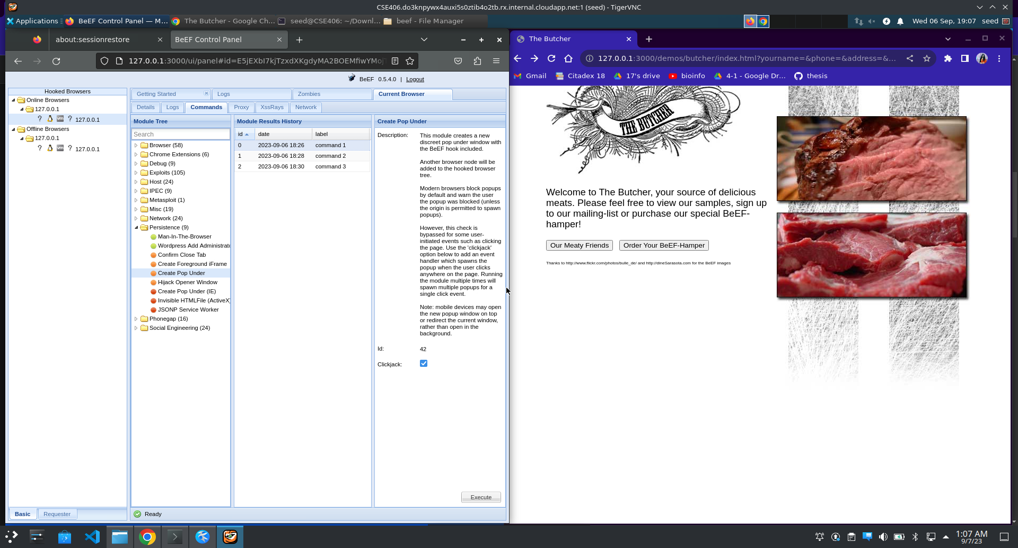
\includegraphics[width=0.8\textwidth]{Create Pop Under/1.png}
    \caption{Creates a new discreet pop under window with BeEF hook included and thus another browser node will be added to the hooked browser tree}
    \label{fig:cpu1}
\end{figure}

\begin{figure}[!htbp]
    \centering
    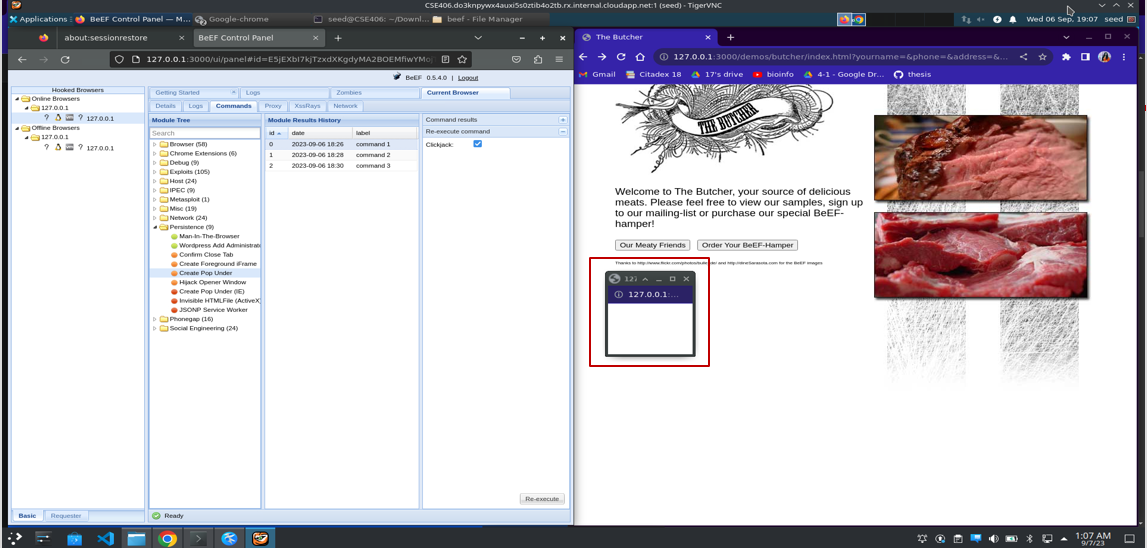
\includegraphics[width=0.8\textwidth]{Create Pop Under/2.png}
    \caption{New window opens}
    \label{fig:cpu2}
\end{figure}

\pagebreak

\subsection{Code}
\begin{figure}[!htbp]
    \centering
    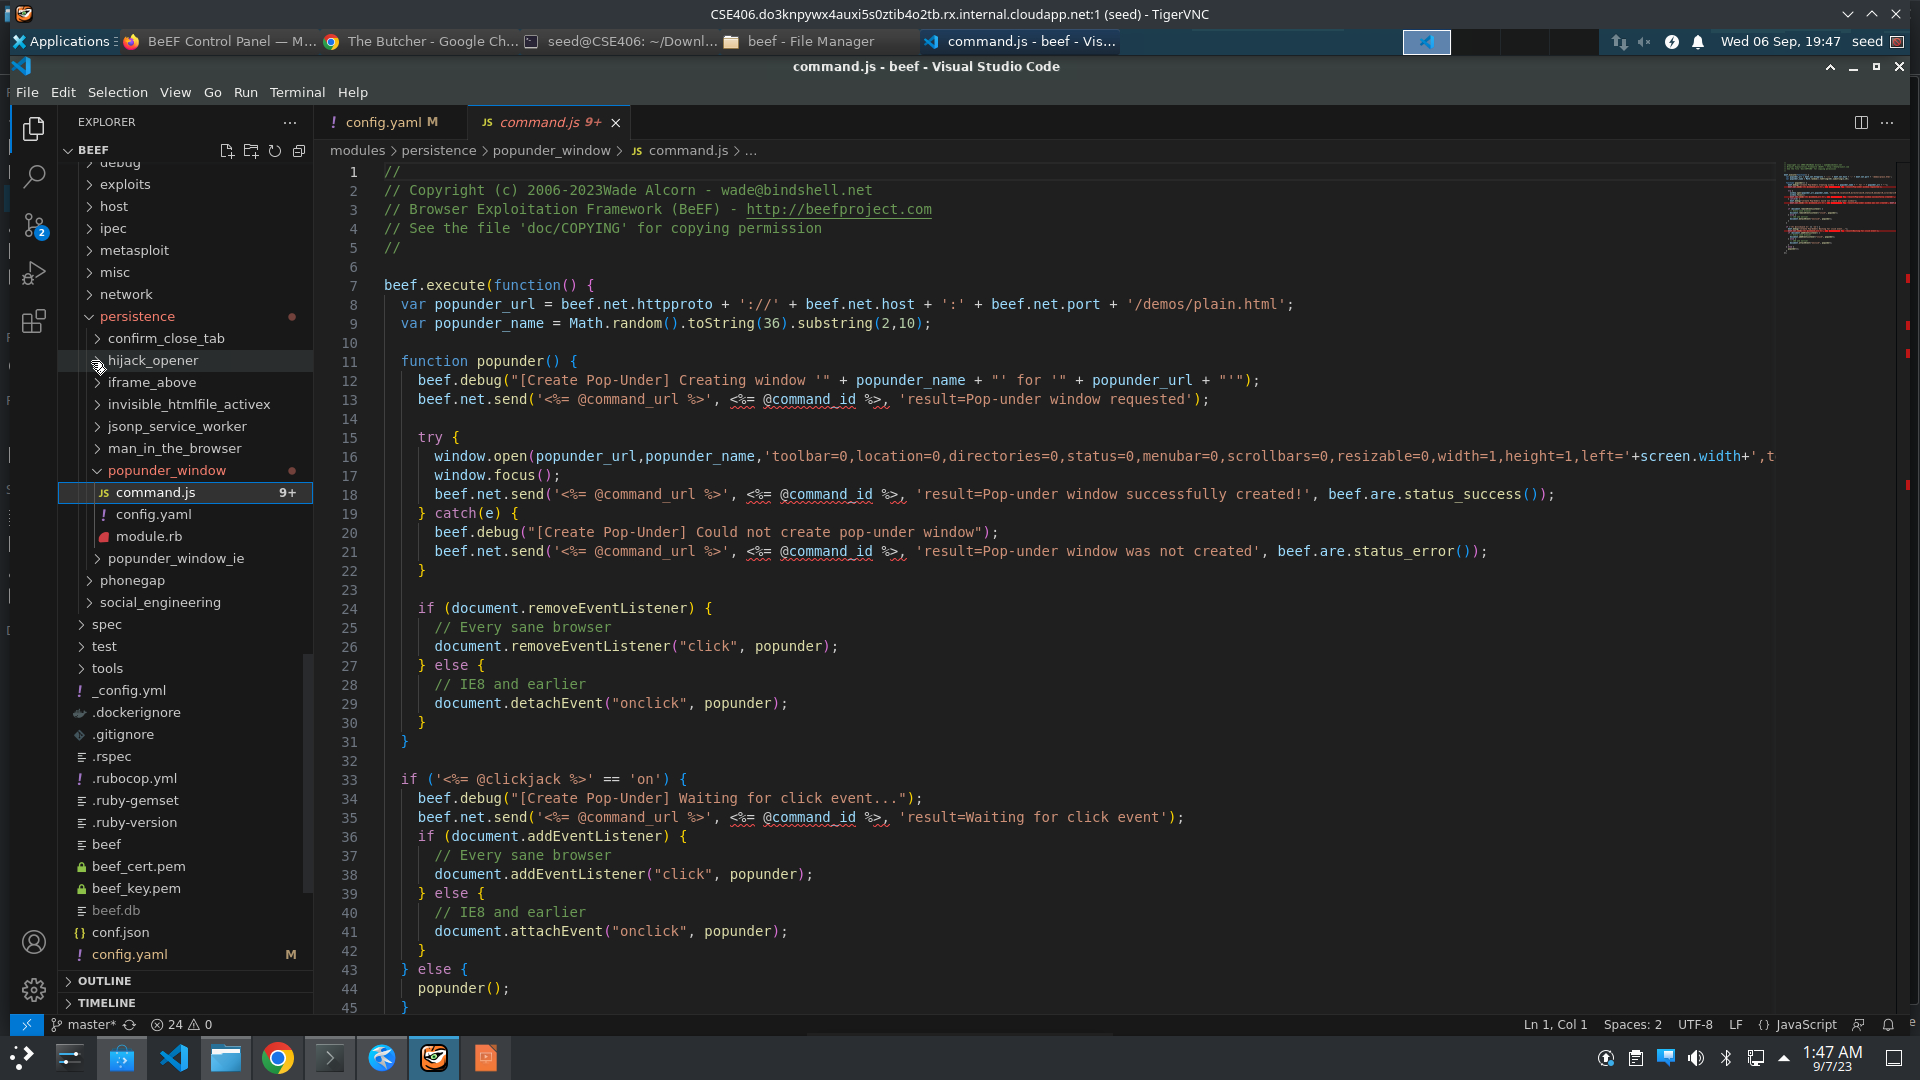
\includegraphics[width=0.8\textwidth]{Create Pop Under/code.png}
    \caption{Code}
    \label{fig:cpu3}
\end{figure}

\pagebreak

\section{ClickJacking}
\subsection{Demonstration}

\begin{figure}[!htbp]
    \centering
    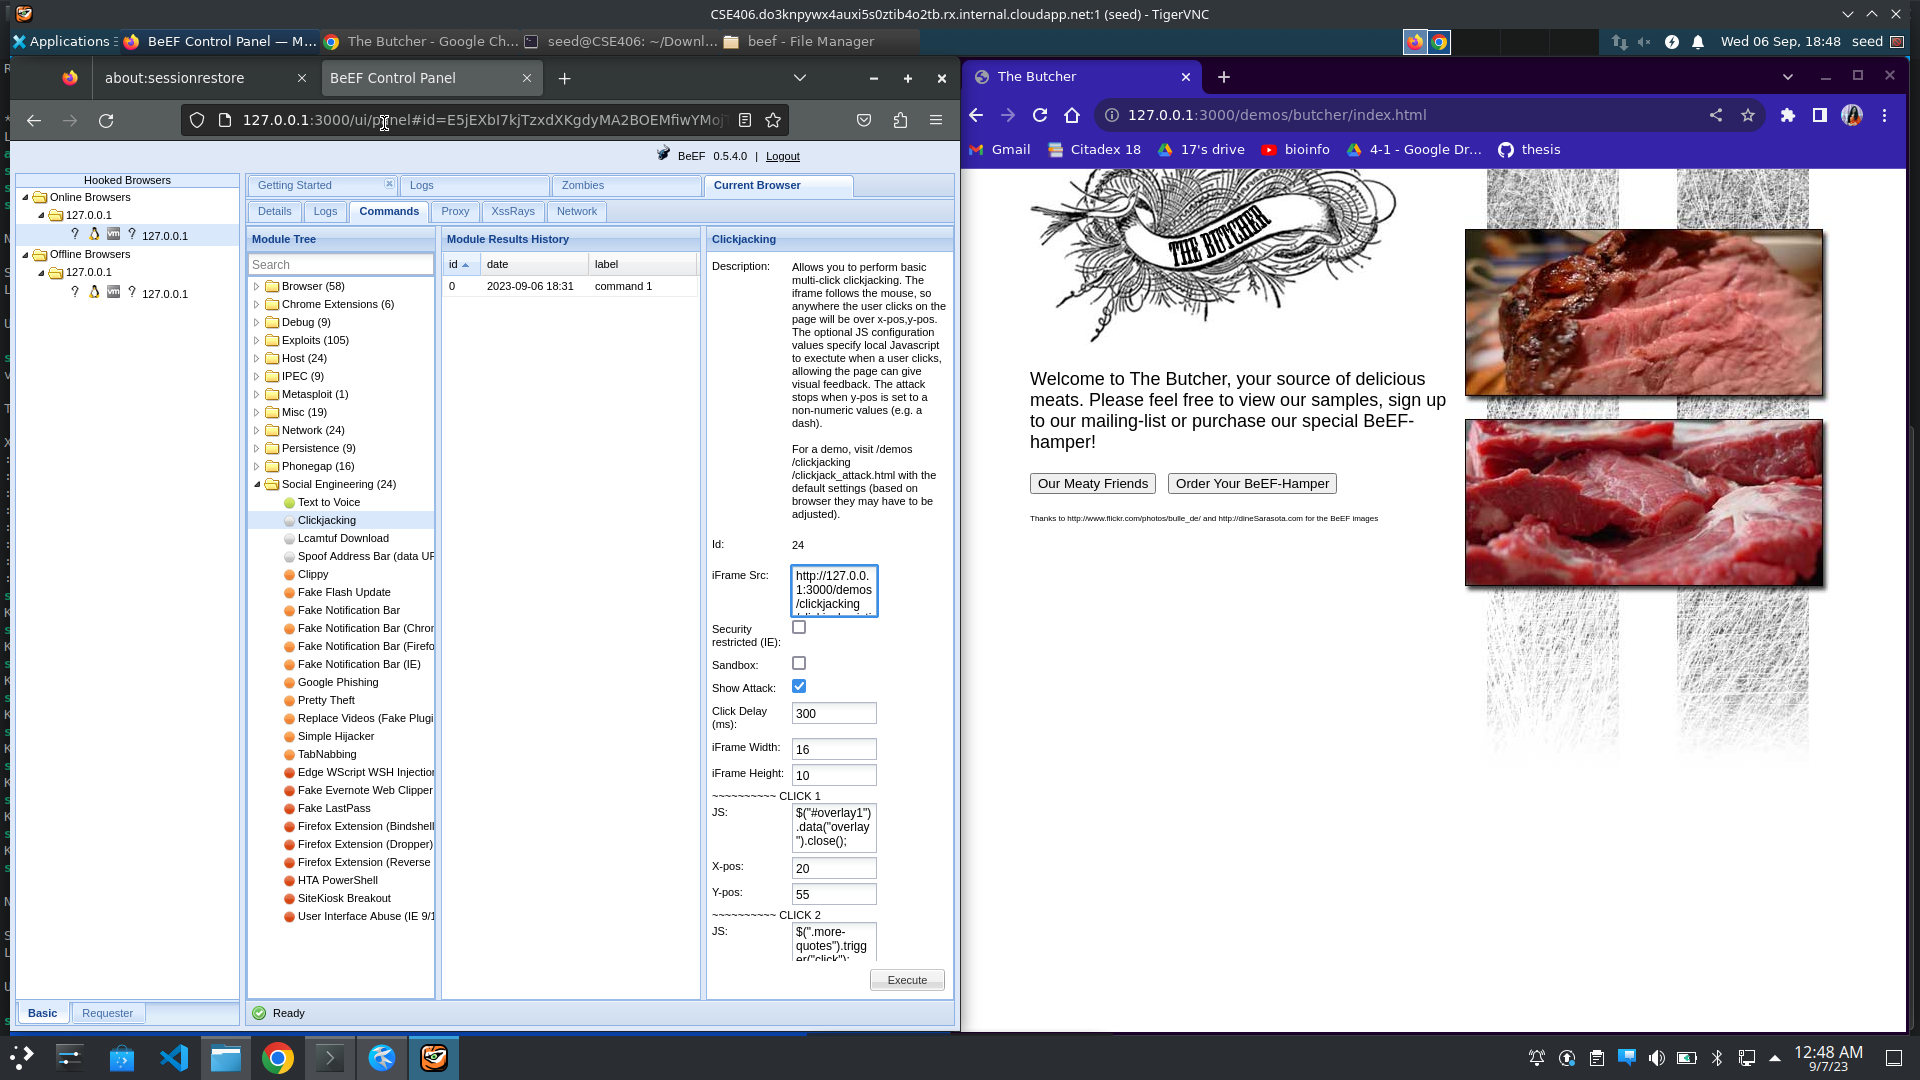
\includegraphics[width=0.8\textwidth]{ClickJacking/1.png}
    \caption{Redirecting to new url while clicking mouse}
    \label{fig:cj1}
\end{figure}

\begin{figure}[!htbp]
    \centering
    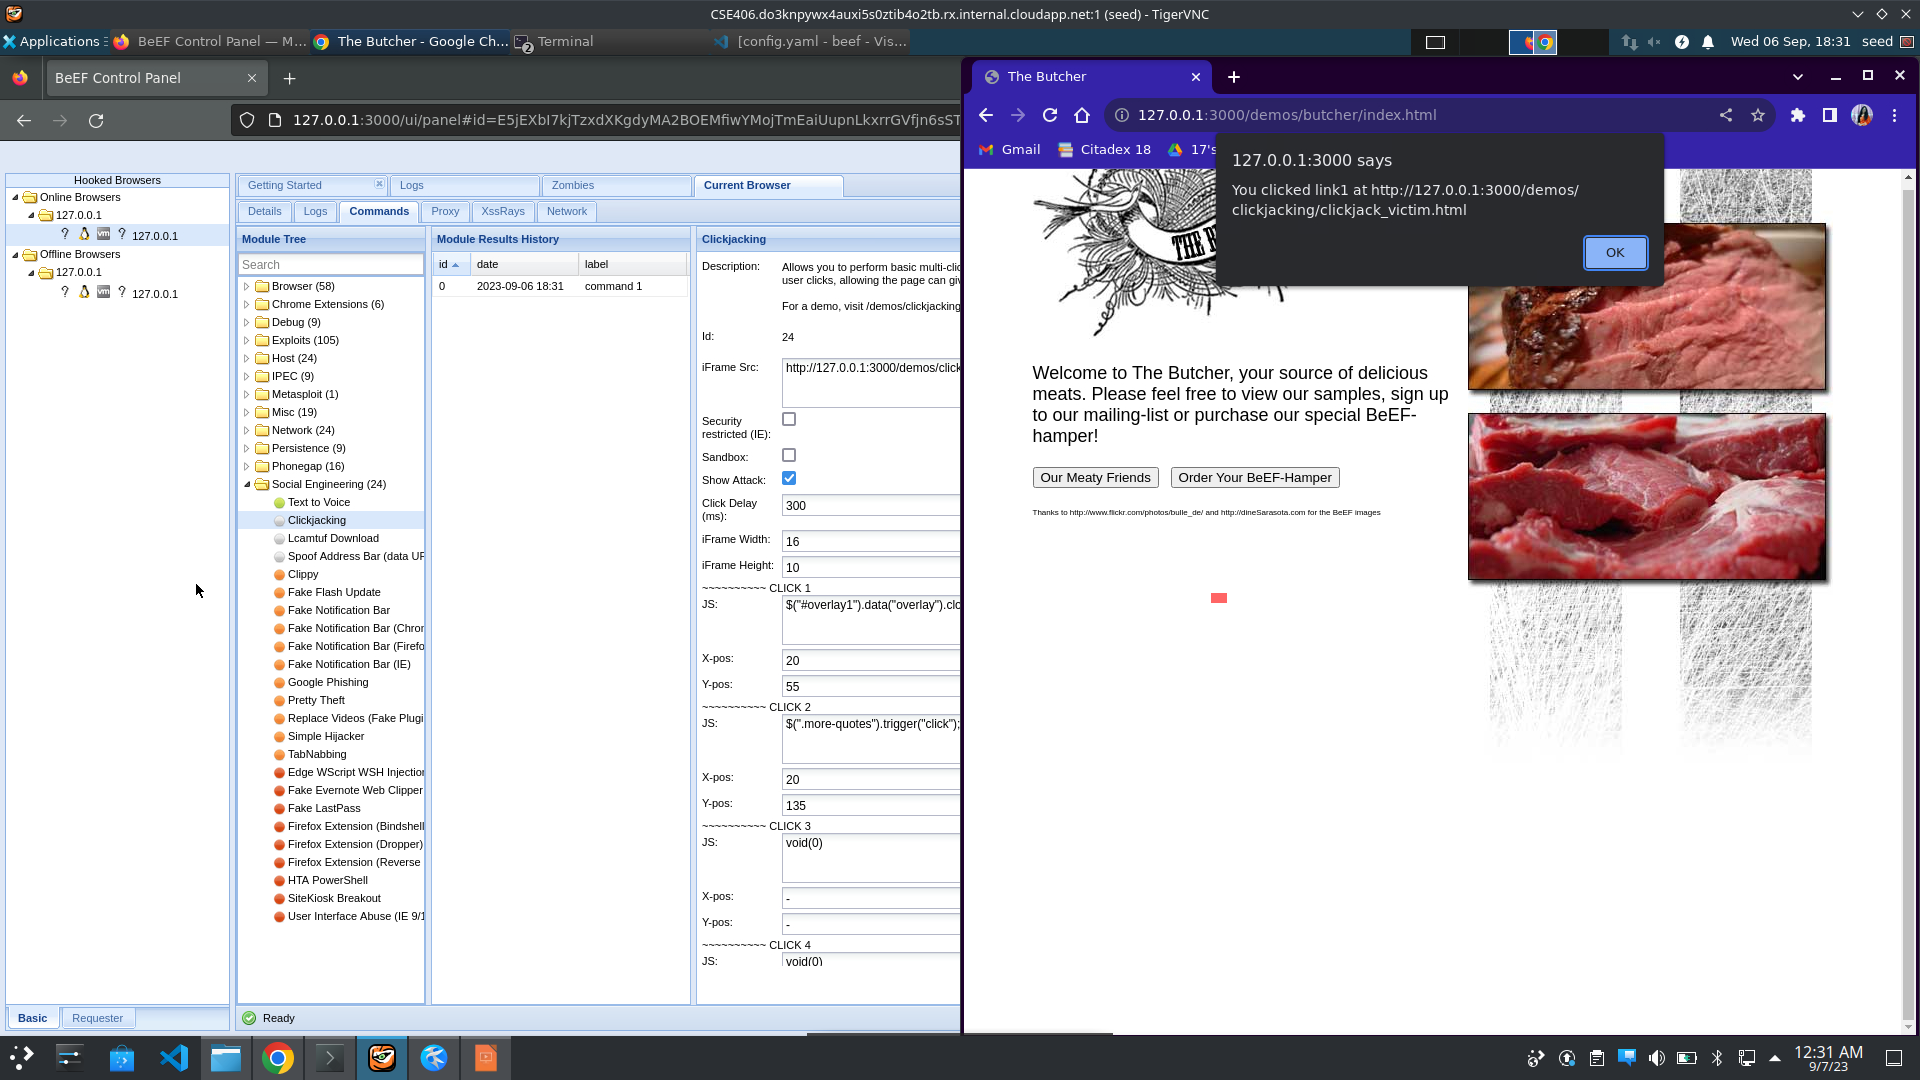
\includegraphics[width=0.8\textwidth]{ClickJacking/2.png}
    \caption{Notification sent}
    \label{fig:cj2}
\end{figure}

\pagebreak

\subsection{Code}
\begin{figure}[!htbp]
    \centering
    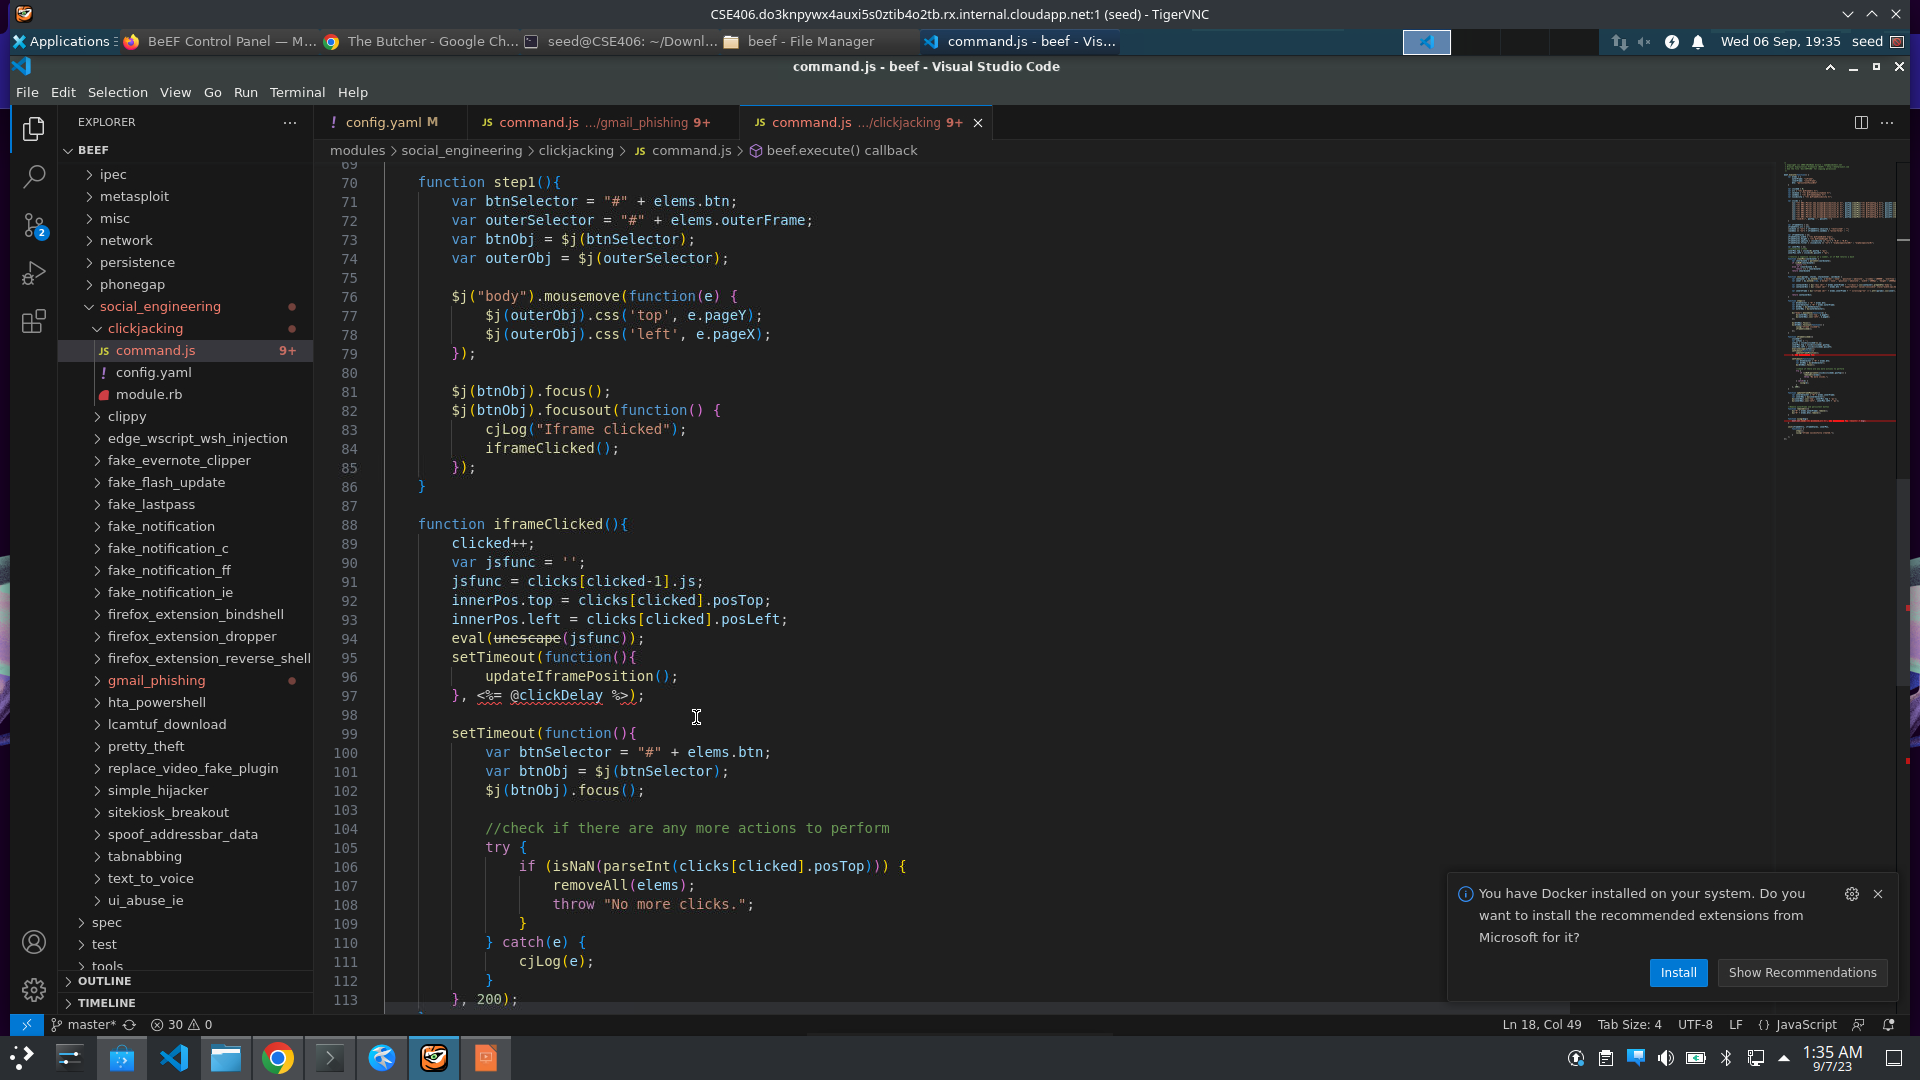
\includegraphics[width=0.8\textwidth]{ClickJacking/code.png}
    \caption{Code}
    \label{fig:cj3}
\end{figure}

\pagebreak


\end{document}